% !TEX root = /home/eb/.vscode/extensions/qftrules.programme-colle/tmp/Exercice.tex

%%%%%%%%%%%%%%%%%%%%%%%%%%%%%%%%%%%
\begin{exo}[PC][3][python]{Diffusion d’un traceur à partir d’un centre}
  \Notions{\item Diffusion \task Solution auto-similaire \task Marche aléatoire}
  On étudie la diffusion des particules d’un traceur (goutte de colorant) dans un liquide contenu dans une cuve de section $S$ et d’axe $(Ox)$. On note $p(x,t)$ la densité de probabilité linéique de trouver une particule de traceur en $x$ à l’instant $t$. On suppose qu’à l’instant initial $t=0$, un nombre $N_0$ de particules de traceur est instantanément déversé au milieu de la cuve, en $x=0$. On note $D$ le coefficient de diffusion.

  \begin{quest}
    \item Écrire l’équation de diffusion particulaire portant sur la fonction $p(x,t)$.
     \sol{
      L’équation de diffusion est 
      \eqbox{
        \frac{\partial p}{\partial t} = D \frac{\partial^2 p}{\partial x^2}.
      }
    }
    \item On cherche une solution de la forme $p(x,t)= A(t) \, e^{-x^2/4Dt}$. Déterminer la fonction $A(t)$ sachant que la densité $p(x,t)$ est normalisée. Vérifier que $p(x,t)$ est bien solution de l’équation de diffusion.
    \sol{
      La normalisation de la densité de probabilité impose 
      $$
      \int_{-\infty}^{+\infty} p(x,t) \d x = 1,
      $$
      soit 
      $$
      \int_{-\infty}^{+\infty} A(t) e^{-x^2/4Dt} \d x = A(t) \sqrt{4 \pi D t} = 1.
      $$
      On en déduit 
      \eqbox{
        A(t) = \frac{1}{\sqrt{4 \pi D t}}.
      }
      
      On calcule 
      $$
      \frac{\partial p}{\partial t} = -\frac{1}{2} (4 \pi D)^{-1/2} t^{-3/2} e^{-x^2/4Dt} + \frac{1}{\sqrt{4 \pi D t}} \times \frac{x^2}{4 D t^2} e^{-x^2/4Dt},
      $$
      et 
      $$
      \frac{\partial^2 p}{\partial x^2} = \frac{1}{\sqrt{4 \pi D t}} \left( \frac{x^2}{4 D^2 t^2} - \frac{1}{2 D t} \right) e^{-x^2/4Dt}.
      $$
      On en déduit 
      $$
      D \frac{\partial^2 p}{\partial x^2} = -\frac{1}{2} (4 \pi D)^{-1/2} t^{-3/2} e^{-x^2/4Dt} + \frac{1}{\sqrt{4 \pi D t}} \times \frac{x^2}{4 D t^2} e^{-x^2/4Dt},
      $$
      ce qui montre que $p(x,t)$ est bien solution de l’équation de diffusion.
    }
    \item La densité particulaire $n(x,t)$ est proportionnelle à la densité de probabilité $p(x,t)$. Déterminer la densité particulaire à l'origine $n_0(t) = n(x=0,t)$ en fonction de $N_0$, $S$, $D$ et $t$. Tracer le graphe de la fonction $x \mapsto n(x,t)$ pour différents instants $t$. Commenter.
    \sol{
      Notons $B$ le coeffecient de proportionnalité. La conservation du nombre total de particules impose
      $$
       N_0 = \int_{\rm cuve} \d N = \int_{\rm cuve} n(x,t) \d V =  B S \int_{-\infty}^{+\infty} p(x,t) \d x =  BS.
      $$
      On en déduit 
      \eqbox{
      n_0(t) = \frac{N_0}{S} A(t) = \frac{N_0}{2S\sqrt{\pi Dt}}.
      }
      
      Le graphe de la fonction $n(x,t)$ à différents instants est celui d’une gaussienne. On constate que la distribution de particules s’étale au cours du temps, avec une hauteur qui diminue. La diffusion tend à homogénéiser la concentration en traceur dans le liquide.
          % \begin{fig}[diffusion]
      %   \centering
      %   \includegraphics[scale=0.6]{diffusion_traceur.png}
      %   %\capt{}
      % \end{fig}
    }
    \item Calculer la distance quadratique moyenne $\delta(t) = \sqrt{\moy{x^2}}$, où $\moy{\cdot}$ désigne la moyenne spatiale. Comparer à la loi d'échelle de la diffusion.
    \sol{
      On a 
      $$
      \moy{x^2} = \int_{-\infty}^{+\infty} x^2 p(x,t) \d x  = \int_{-\infty}^{+\infty} x^2 \frac{1}{\sqrt{4 \pi D t}} e^{-x^2/4Dt} \d x = 2 D t.
      $$
      On en déduit 
      \eqbox{
        \delta(t) = \sqrt{2 D t}.
      }
      
      La distance quadratique moyenne croît comme la racine carrée du temps, caractéristique d’un processus diffusif.
    }
  \end{quest}

  \textsc{Données} : $\int_{-\infty}^{+\infty} e^{-a x^2} \d x = \sqrt{\pi/a}$ ; $\int_{-\infty}^{+\infty} x^2 e^{-a x^2} \d x = \frac{1}{2 a} \sqrt{\pi/a}$.

  On simulera numériquement la diffusion du traceur dans le liquide en utilisant un modèle de marche aléatoire. Voir la \refCN{3}, dont le lien \texttt{Capytale} est le suivant :
  \begin{center}
    \href{https://capytale2.ac-paris.fr/p/basthon/n/?kernel=python3-legacy\&mode=create\&id=4545039}{https://capytale2.ac-paris.fr/p/basthon/n/?kernel=python3-legacy\&mode=create\&id=4545039}
  \end{center}
  
\end{exo}
%%%%%%%%%%%%%%%%%%%%%%%%%%%%%%%%%%%

\begin{exo}[PC][1][python]{Tutorat 1}
    
  % \section*{II. 2 - }
  \parag{Introduction}
  

  De nombreux procédés industriels font intervenir des réacteurs fermés pour la synthèse de molécules à haute valeur ajoutée. Pour optimiser le rendement de la synthèse, il est nécessaire de bien comprendre l'influence des paramètres physiques (comme la température de la réaction,...) sur la marche du réacteur. La maîtrise des échanges thermiques est cruciale dans le cas des réactions exothermiques car la chaleur dégagée par la réaction provoque une augmentation de la température du mélange réactionnel. Selon les conditions opératoires, cette augmentation de température peut entraîner un emballement thermique du réacteur et conduire à des dégâts irréversibles.


  Nous utiliserons un modèle d'évolution du taux de conversion du réactif \(X_{R}\) et de la température de réaction \(T\) en fonction du temps pour prédire le comportement thermique du réacteur en présence d'une réaction exothermique. Dans ce modèle, les grandeurs \(X_{R}\) et \(T\) vérifient les équations différentielles suivantes :
\begin{equation}
  \left\{\begin{array}{l}
    \frac{d X_{R}}{d t}=f_{1}\left(t, X_{R}, T\right), \text{ avec } f_1(t,X_R,T) =  -k_0 \exp \left( - E_a / R T\right) \left(X_R-1\right), \\[0.3cm]
    \frac{d T}{d t}=f_{2}\left(t, X_{R}, T\right), \text{ avec } f_2(t,X_R,T) =  J \dd{X_R}{t}-\frac{T-T_p}{\tau_c}. \\[0.3cm]
  \end{array}\right.
\end{equation}
où $k_0$ est la constante de réaction à température infinie, $E_a$ est l'énergie d'activation, $R$ la constante des gaz parfaits, $J$ et $T_p$ sont des températures caractéristiques, et $\tau_c$ un temps caractéristique.

\parag{Schéma numérique}

La méthode de résolution proposée pour résoudre le système d'équations différentielles est la méthode d'\emph{Euler implicite à pas fixe}. Cette méthode est préférée car elle donne de meilleurs résultats que la méthode explicite pour les systèmes dits raides (un système raide est un système qui est caractérisé par une évolution rapide des phénomènes en fonction du temps, ce qui est le cas ici pour la température de réaction).

Soit une variable \(y\) qui dépend du temps \(t\). Comme la méthode d'Euler explicite, la méthode d'Euler implicite consiste à évaluer la valeur de \(y(t+\Delta t)\) à partir de celle de \(y(t)\) et de la dérivée \(\frac{\partial y}{\partial t}\) (\Fig{euler}). La différence entre les deux méthodes réside dans le choix de l'abscisse à laquelle est évaluée la dérivée \(\frac{\partial y}{\partial t}\). Dans le cas de la méthode explicite, elle est évaluée en \(t: \frac{\partial y}{\partial t}(t)\) comme le montre le schéma de la \Fig{euler_1}. Pour la méthode implicite, elle est évaluée en \(t+\Delta t: \frac{\partial y}{\partial t}(t+\Delta t)\) (\Fig{euler_2}).
\begin{fig}[euler]
  \centering
  \begin{subfig}[euler_1][0.48]
    
\includegraphics[width=\textwidth]{2024_12_09_d77689dc8895c227f186g-02(1)}
  \end{subfig}
  \begin{subfig}[euler_2][0.48]
    
\includegraphics[width=\textwidth]{2024_12_09_d77689dc8895c227f186g-02}
  \end{subfig}
  \capt{Approximation de \(y(t+\Delta t)\) par la méthode d'Euler. (a) Cas de la méthode explicite.  (b) Cas de la méthode implicite.}
\end{fig}
Dans le cas d'un schéma implicite (figure 4b), l'expression de \(y(t+\Delta t)\) en fonction de \(y(t)\) et de la dérivée \(\frac{\partial y}{\partial t}(t+\Delta t)\) évaluée en \(t+\Delta t\) est obtenue en réalisant un développement limité dit rétrograde : 
\begin{equation}
y(t)=y(t+\Delta t)-\Delta t \times \frac{\partial y}{\partial t}(t+\Delta t)+o(\Delta t).
\end{equation}
\begin{quest}
  \item À l'aide d'un développement limité rétrograde de la fonction \(X_{R}(t)\), donner l'expression de \(X_{R}(t+\Delta t)\) à l'ordre 1 en fonction de \(X_{R}(t)\) et de sa dérivée partielle par rapport à \(t\), \(\frac{d X_{R}}{d t}(t+\Delta t)\) évaluée en \(t+\Delta t\).
  \sol{
    On a
$$    X_R(t)=X_R(t+\Delta t)-\Delta t \dd{X_R}{t}(t+\Delta t)+o(\Delta t),
$$
et donc
    \eqbox{
      X_R(t+\Delta t)=X_R(t)+\Delta t \dd{X_R}{r}(t+\Delta t)+o(\Delta t)
    }  
  }
  
  \item En déduire une valeur approchée de \(\frac{d X_{R}}{d t}(t+\Delta t)\) à l'ordre 0 en fonction de \(X_{R}(t)\), \(X_{R}(t+\Delta t)\) et \(\Delta t\).
  \sol{
  \eqbox{
    \dd{X_R}{t}(t+\Delta t)=\frac{X_R(t+\Delta t)-X_R(t)}{\Delta t} + o(1)
  }
  }
  
  \item À l'aide d'un développement limité rétrograde de la fonction \(T(t)\), donner l'expression de \(T(t+\Delta t)\) à l'ordre 1 en fonction de \(T(t)\) et de sa dérivée partielle par rapport à \(t, \frac{d T}{d t}(t+\Delta t)\).
  \sol{
  De même, on a 
  \eqbox{
    T(t+\Delta t)=T(t)+\Delta t  \dd{T}{t}(t+\Delta t)+o(\Delta t).
    }
  
  }
  
  \item En déduire une valeur approchée de \(\frac{d T}{d t}(t+\Delta t)\) à l'ordre 0 en fonction de \(T(t), T(t+\Delta t)\) et \(\Delta t\).
  \sol{
    Et donc 
    \eqbox{
      \dd{T}{t}(t+\Delta t)=\frac{T(t+\Delta t)-T(t)}{\Delta t} + o(1).
    }
  }
\end{quest}

On procède à la discrétisation des équations. On note \(X_{R i}\) la conversion évaluée au temps \(t_{i}, X_{R i+1}\) la conversion évaluée au temps \(t_{i+1}\) et \(\left.\frac{d X_{R}}{d t}\right|_{t_{i+1}}\) la dérivée de \(X_{R}\) évaluée à l'instant \(t_{i+1}\). De même, on note \(T_{i}\) la température évaluée au temps \(t_{i}, T_{i+1}\) la température évaluée au temps \(t_{i+1}\) et \(\left.\frac{d T}{d t}\right|_{t_{i+1}}\) la dérivée de \(T\) évaluée à l'instant \(t_{i+1}\).
\begin{quest}
  
  \item Donner l'expression de \(\left.\frac{d X_{R}}{d t}\right|_{t_{i+1}}\) en fonction de \(X_{R i}, X_{R i+1}\) et \(\Delta t\).
  \sol{
  On a $t_i = i \Delta t$ et $t_{i+1} = (i+1) \Delta t = t_i + \Delta t$. D'après les résultats des questions précédentes, on a donc
  \eqbox{
    \left.\frac{d X_R}{d t}\right|_{t_{i+1}}=\frac{X_{R_{i+1}}-X_{R_i}}{\Delta t}
  }
  }
  \item Donner l'expression approchée de \(X_{R i+1}\) en fonction de \(X_{R i}, \Delta t\) et de la fonction \(f_{1}\left(t_{i+1}, X_{R i+1}, T_{i+1}\right)\), évaluée en \(t_{i+1}\).
  \sol{
  L'équatino différentielle qui porte sur $X_R$ est 
  $$
  \dd{X_R}{t} = f_1(t, X_R, T).
  $$
  La version discrétisée de cette équation à l'ordre $1$ est donc 
  \eqbox{
    X_{R_{i+1}}=X_{R_i}+\Delta t f_1\left(t_{i+1}, X_{R i+1}, T_{i+1}\right)
  }
  }
  
  \item Donner l'expression de \(\left.\frac{d T}{d t}\right|_{t_{i+1}}\) en fonction de \(T_{i}, T_{i+1}\) et \(\Delta t\).
  \sol{
  De même,
  \eqbox{
    \left.\dd{T}{t}\right|_{t_{i+1}}=\frac{T_{i+1}-T_i}{\Delta t}.
  }
  }
  
  \item Donner l'expression approchée de \(T_{i+1}\) en fonction de \(T_{i}, \Delta t\) et de la fonction \(f_{2}\left(t_{i+1}, X_{R i+1}, T_{i+1}\right)\), évaluée en \(t_{i+1}\).
  \sol{
  De même,
  \eqbox{
    T_{i+1}=T_i+\Delta t f_2\left(t_{i+1}, X_{R i+1} T_{i+1}\right).
  }
  }
\end{quest}
  
\parag{Implémentation du schéma numérique}

  On constate que les expressions obtenues aux questions \(\mathbf{Q 3 2}\) et \(\mathbf{Q 3 4}\) constituent un système non linéaire dont les inconnues sont \(X_{R i+1}\) et \(T_{i+1}\). On propose d'utiliser la méthode de Newton-Raphson pour trouver les valeurs de \(X_{R i+1}\) et \(T_{i+1}\) à chaque itération de la méthode d'Euler.
  
  La méthode de Newton-Raphson pour la résolution d'un système de \(n\) équations non linéaires à \(n\) inconnues \(x=\left(x_{1}, \ldots, x_{n}\right)\), mis sous la forme suivante,

% \[
\begin{equation}
  g(x)=\left[\begin{array}{c}
    g_{1}\left(x_{1}, \ldots, x_{n}\right) \\
    \ldots \\
    g_{n}\left(x_{1}, \ldots, x_{n}\right)
  \end{array}\right]= 0
\end{equation}
% \]

est une extension de la méthode de Newton permettant de trouver la racine d'une fonction d'une variable.

On peut démontrer la formule de récurrence suivante :

% \[
\begin{equation}\label{eq:recur}
  x^{j+1}=x^{j}-\left[D g\left(x^{j}\right)\right]^{-1} g\left(x^{j}\right)
\end{equation}
% \]

où \(x^{j+1}\) est la valeur du vecteur \(x\) à l'itération \(j+1, x^{j}\) est la valeur du vecteur \(x\) à l'itération \(j\), \(g\left(x^{j}\right)\) est la valeur de \(g(x)\) à l'itération \(j\) et \(D g\left(x^{j}\right)\) est la matrice Jacobienne évaluée en \(x^{j}\) :

% \[
\begin{equation}
  D g\left(x^{j}\right)=\left[\begin{array}{ccc}
    \frac{\partial g_{1}}{\partial x_{1}} & \cdots & \frac{\partial g_{1}}{\partial x_{n}} \\
    \ldots & & \cdots \\
    \frac{\partial g_{2}}{\partial x_{1}} & \ldots & \frac{\partial g_{2}}{\partial x_{n}}
  \end{array}\right]_{x=x^{j}}
\end{equation}
% \]

La formule de récurrence s'accompagne du choix d'une valeur initiale, notée \(x^{0}\), et d'un critère d'arrêt, par exemple \(\left\|x^{j+1}-x^{j}\right\| \leq \varepsilon\).

Les algorithmes demandés au candidat devront être réalisés dans le langage Python. On supposera les bibliothèques « numpy » et « matplotlib.pyplot » chargées. Une annexe présentant les fonctions usuelles de Python est disponible pages 15 à 18 . Les commentaires suffisants à la compréhension du programme devront être apportés et des noms de variables explicites devront être utilisés lorsque ceux-ci ne sont pas imposés.

\begin{quest}
  \item Transformer les expressions obtenues aux questions pour les mettre sous la forme \(g_{1}\left(X_{R i+1}, T_{i+1}\right)=0\) et \(g_{2}\left(X_{R i+1}, T_{i+1}\right)=0\).
  \sol{
  On trouve 
  \eqbox{
    g_1\left(X_{R_{i+1}}, T_{i+1}\right)=X_{R_{i+1}}-X_{R_i}+k_0 \Delta t \exp \left(-E_a / R T_{i+1}\right) \left(X_{R_{i+1}}-1\right)=0,
  }
  et 
  \eqbox{
    g_2\left(X_{R_{i+1}}, T_{i+1}\right)=T_{{i+1}}-T_{i} - J k_0 \exp \left(-E_a / R T_{i+1}\right) \left(X_{R_{i+1}}-1\right) \Delta t-\frac{T_{i+1}-T_p}{\tau_c} \Delta t=0.
  }
  }
  
  \item Donner les expressions de \(\frac{\partial g_{1}}{\partial X_{R i+1}}, \frac{\partial g_{1}}{\partial T_{i+1}}, \frac{\partial g_{2}}{\partial X_{R i+1}}\) et \(\frac{\partial g_{2}}{\partial T_{i+1}}\) permettant de construire la matrice Jacobienne \(\operatorname{Dg}\left(X_{R i+1}, T_{i+1}\right)\).
  \sol{
    On a
   $$ \begin{aligned}
      & \frac{\partial g_1}{\partial X_{R_{i+1}}}=1+k_0 \Delta t \exp \left(-E_a / R T_{i+1}\right)\\
      &\begin{aligned}
      & \frac{\partial g_1}{\partial T_{i+1}}=k_0 \Delta t\left(+\frac{E_a}{R T_{i+1}^2}\right) \exp \left(-E_a / R T_{i+1}\right) \times\left(X_{R i+1}-1\right) \\
      & \frac{\partial g_2}{\partial X_{R_{i+1}}}=\Delta t J k_0 \exp \left(-E_a / R T_{i+1}\right) \\
      & \frac{\partial g_2}{\partial T_{i+1}}=1+J k_{0} \frac{E_a}{R T_{i+1}} \exp \left(-E_a / R T_{i+1}\right) \times\left(X_{R_{i+1}}-1\right)-\frac{\Delta t}{\tau_c}
      \end{aligned}
      \end{aligned}$$
  }
  \item Écrire une fonction \texttt{mat\_Dg(x)} qui a pour argument d'entrée un vecteur \(x\) contenant les valeurs de \(X_{R i+1}\) et \(T_{i+1}\) à l'itération \(j\) et qui retourne la matrice Jacobienne \(D g\left(x^{j}\right)\). On supposera que les paramètres suivants ont été au préalable déclarés comme variables globales : \(\Delta t=0,01 \mathrm{~s}\), \(k_{0}=5,0 \mathrm{~s}^{-1}, E_{a}=20000,0 \mathrm{~J} . \mathrm{mol}^{-1}, J=100,0 \mathrm{~K}, \tau_{c}=75 \mathrm{~s}\) et \(R=8,314 \mathrm{~J} \cdot \mathrm{~K}^{-1} \cdot \mathrm{~mol}^{-1}\).
  \sol{
   Je suppose déjà créés les fonctions $g_1 T=\frac{\partial g_1}{\partial T_{i+1}}, g_1 X=\frac{\partial g_1}{\partial x_{i+1}}$ $g_2 T=\frac{\partial g_2}{\partial T_{i+1}}$ et $g_2 X=\frac{\partial g_2}{\partial X_{k i+1}}$, aimi que $g_1$ er $g_2$. On définit le vecteur $x=(X_{R},T)$.
  %  \begin{verbatim}
  \inputminted{python}{/home/eb/Dropbox/CPGE/Physique/Exercices/Recueil/Thermo/Code/mat_Dg.py}
  %  \begin{minted}{python}
    % def mat_Dg(x)
    %   Dg=np.zeros((2,2)) 
    %   Dg[0,0]=g_1 T(x[0], x[1]) 
    %   Dg[0,1]=g_1 x(x[0], x[1]) 
    %   Dg[1,0]=g_2 T(x[0], x[1]) 
    %   Dg[1,1]=g_2 x(x[0], x[1])
    %   return Dg
    % \end{minted}
    % \end{verbatim}
  }
  
  \item Écrire le code permettant de calculer les valeurs du vecteur \(x\) à l'itération \(j+1\) à l'aide de l'\Eq{recur} lors d'une boucle de l'algorithme de Newton-Raphson. On notera x\_old la valeur de \(x\) à l'itération \(j\) et \(\mathbf{x} \_\)new la valeur de \(x\) à l'itération \(j+1\). De même, on notera x\_euleri et T\_euleri les vecteurs contenant les valeurs de \(X_{R i}\) et \(T_{i}\) à l'itération \(i\) de la méthode d'Euler implicite. Pour l'inversion de matrice, on utilisera la fonction \texttt{inv\_mat(M)} qu'on suppose être prédéfinie.
  
  \sol{
    \inputminted{python}{/home/eb/Dropbox/CPGE/Physique/Exercices/Recueil/Thermo/Code/inv_Dg.py}
  }
  \item Pour obtenir la valeur de x\_new par la méthode de Newton-Raphson, on souhaite créer une boucle itérative avec condition. La condition d'arrêt porte sur la valeur absolue de la différence des températures \(T_{i+1}^{j}\) et \(T_{i+1}^{j+1}\) que l'on souhaite inférieure à \(10^{-5} \mathrm{~K}\). Pour les valeurs initiales de \(X_{R i+1}^{0}\) et \(T_{i+1}^{0}\) on prendra respectivement 0,5 et \(T_{p}+J / 2\). Écrire le code correspondant. Il est inutile de recopier l'intégralité du code écrit à la question précédente ; on indiquera néanmoins sa place dans le code de cette question.
  \sol{
    \inputminted{python}{/home/eb/Dropbox/CPGE/Physique/Exercices/Recueil/Thermo/Code/boucle_Dg.py}
  }
\end{quest}
  
  Maintenant que le code permettant de trouver les valeurs de \(X_{R i+1}\) et \(T_{i+1}\) par la méthode de Newton-Raphson lors d'une itération de la méthode d'Euler implicite a été établi, on souhaite calculer les valeurs pour l'ensemble des itérations de la méthode d'Euler implicite. On rappelle que \(X_{R}(t=0)=0\) et \(T(t=0)=T_{p}=320,0 \mathrm{~K}\). En plus de noter \(\mathbf{x} \_\)euleri et \(\mathbf{T} \_\)euleri les vecteurs contenant les valeurs de \(X_{R i}\) et \(T_{i}\) pour chaque itération \(i\) de la méthode d'Euler implicite, on notera t\_euleri le vecteur contenant les valeurs de \(t_{i}\) à chaque itération. L'intégration sera réalisée sur l'intervalle \(\left[t_{0}, t_{f}\right]\) avec \(t_{0}=0 \mathrm{~s}\) et \(t_{f}=1000 \mathrm{~s}\). Le pas de temps \(\Delta t\) est de \(0,01 \mathrm{~s}\).

  \begin{quest}
      \item Donner le code permettant de calculer le nombre \(m\) d'intervalles \(\Delta t\) compris dans l'intervalle \(\left[t_{0}, t_{f}\right]\) ( \(m\) est un entier).
      \sol{
        \inputminted{python}{/home/eb/Dropbox/CPGE/Physique/Exercices/Recueil/Thermo/Code/m_Dg.py}
      }
      \item Écrire le code permettant de calculer les valeurs des éléments des vecteurs x\_euleri, T\_euleri et t\_euleri à chaque itération de la méthode d'Euler implicite.
      \sol{
        \inputminted{python}{/home/eb/Dropbox/CPGE/Physique/Exercices/Recueil/Thermo/Code/all_Dg.py}
      }
      \item Donner le code permettant de tracer les graphes de la \Fig{graphe_TX} montrant l'évolution de la conversion et de la température en fonction du temps que l'on obtiendrait en réalisant la résolution numérique du système d'équations différentielles (simulation réalisée avec $k_0=5,0 \mathrm{~s}^{-1}$, $E_a=20000,0 \mathrm{~J} \cdot \mathrm{~mol}^{-1}$, $J=100,0 \mathrm{~K}$, $\tau_c=75 \mathrm{~s}$).
      \sol{
        \inputminted{python}{/home/eb/Dropbox/CPGE/Physique/Exercices/Recueil/Thermo/Code/plot_Dg.py}
      }
  \end{quest}
\begin{fig}[graphe_TX]
  \centering
  \begin{subfig}[label][0.48]
    
\includegraphics[width=\textwidth]{2024_12_09_d77689dc8895c227f186g-05_1.jpg}
  \end{subfig}
  \begin{subfig}[label][0.48]
    
\includegraphics[width=\textwidth]{2024_12_09_d77689dc8895c227f186g-05_2.jpg}
  \end{subfig}
  \capt{Température et conversion calculées à partir du modèle constitué du système d'équations différentielles.}
\end{fig}

\end{exo}
%%%%%%%%%%%%%%%%%%%%%%%%%%%%%%%%%%%

%%%%%%%%%%%%%%%%%%%%%%%%%%%%%%%%%%%
\begin{exo}[PC][1][TD]{Transport d'oxygène sanguin}
  \Notions{\item Ordre de grandeur \task Coefficient de diffusion}
  Une des fonctions du sang est le transport de dioxygène depuis le poumon vers les organes. Le sang se charge en oxygène par diffusion du gaz contenu dans les alvéoles pulmonaires, supposées sphériques de rayon $R \simeq \SI{100}{\mu m}$, vers le capillaire sanguin, qui longe un côté de l'alvéole. Le sang circule dans un capillaire de rayon $r \simeq \SI{10}{\mu m}$ à la vitesse $v \simeq \SI{1e-3}{m.s^{-1}}$. On note $D_{\text {air }} \simeq \SI{2e-5}{m^2.s^{-1}}$ le coefficient de diffusion du dioxygène dans l'air et $D_{\text {eau }} \simeq \SI{1e-9}{m^2.s^{-1}}$ celui du dioxygène dans un milieu aqueux comme le sang.

  \begin{fig}[label]
    \centering
    
\includegraphics[scale=0.65]{alveole.pdf}
    %\capt{}
  \end{fig}
  \begin{quest}
    \item Rappeler la définition du coefficient de diffusion. Commenter les valeurs de $D_{\text {air}}$ et $D_{\text {eau}}$.
    \item Schématiser l'alvéole et le capillaire sanguin. Déterminer le temps de contact $t_{\rm c}$ entre le sang du capillaire et l'alvéole pulmonaire. 
    \item Déterminer le temps total de diffusion $t_{\rm d}$ du dioxygène à travers l'alvéole pulmonaire et le capillaire sanguin. Comparer à $t_{\rm c}$ et conclure.
  \end{quest}
\end{exo}
%%%%%%%%%%%%%%%%%%%%%%%%%%%%%%%%%%%

%%%%%%%%%%%%%%%%%%%%%%%%%%%%%%%%%%%
\begin{exo}[PC][1][python]{Marche aléatoire}
% \inputminted{python}{marche_alea_1.py}
Un modèle de marche aléatoire permet de simuler le déplacement erratique des particules à l'échelle microscopique engendré par l'agitation thermique par exemple. On étudie une particule au milieu de particules voisines, qui se déplace au gré des chocs. On suppose pous simplifier que la particule par de l'origine et effectue un saut de longueur $\ell$ à chaque pas de temps $\tau$. Dans un modèle $1D$ (une dimension), la particule se déplace sur un axe $x$ et peut donc sauter, soit à droite, soit à gauche, avec la même probabilité. On admet que la probabilité $p(x,t)$ que la particule soit à la position $x$ à l'instant $t$ vérifie l'équation de diffusion
% $$
% \boxed{
\begin{equation}
  \frac{\partial p}{\partial t} = D \frac{\partial^2 p}{\partial x^2},
\end{equation}
  % },
% $$
où $D=\textstyle\frac{\ell^2}{2\tau}$ est le coefficient de diffusion.

\begin{quest}
  \item Proposer un schéma de principe de la marche aléatoire $1D$.
  \item	Nous commençons par définir les grandeurs $\ell$, $\tau$ et $D$, puis nous simulons \texttt{N} sauts de la particule. La fonction \texttt{marche} renvoie la position finale de la particule après \texttt{N} sauts. Compléter la ligne pointillée de façon à actualiser la nouvelle position $x$ de la particule après son saut aléatoire, sachant que la fonction \texttt{randint(a,b,...)} de la bibliothèque \texttt{random} renvoie un entier aléatoire parmi $a$, $b$, ...
  \begin{minted}{python}
""" BIBLIOTHEQUES """
import numpy as np
import random as r

""" PARAMETRES """
l   = 1            # distance des sauts
tau = 1            # durée entre sauts
D   = l**2/2/tau   # coefficient de diffusion

""" SIMULATION """
def marche(N):
    x = 0                          # position initiale
    for i in range(N):             # boucle sur les sauts
        x = ...                    # saut
    return x                       # position finale
\end{minted}

% \sol{
  \begin{minted}{python}
    """ BIBLIOTHEQUES """
    import numpy as np
    import random as r
    
    """ PARAMETRES """
    l   = 1            # distance des sauts
    tau = 1            # durée entre sauts
    D   = l**2/2/tau   # coefficient de diffusion
    
    """ SIMULATION """
    def marche(N):
        x = 0                          # position initiale
        for i in range(N):             # boucle sur les sauts
            x = x + l*r.randint(-1,1)  # saut
        return x                       # position finale
    \end{minted}
% }

\item On souhaite lancer un grand nombre de simulations pour obtenir des informations sur la distribution de probabilité de la position de la particule.
Que vaut la moyenne de la position $\moy{x}$ ? Pourquoi est-il plus intéressant d'étudier la distance quadratique moyenne $\moy{x^2}$ ?
\sol{
  La moyenne de la position est nulle, car la particule a autant de chance de sauter à droit qu’à gauche. On a donc $\moy{x}=0$. Pour étudier la distribution de position de la particule, il faut donc étudier l’ordre supérieur : la distance quadratique moyenne $\moy{x^2}$, qui caractérise la dispersion de la particule autour de l’origine.
}
\item 
  Compléter les lignes pointillées ci-dessous. La fonction \texttt{dquad} doit renvoyer la distance quadratique moyenne $\moy{x^2}$ calculée sur $1000$ simulations de \texttt{N} sauts. On pourra utiliser la méthode \texttt{append} pour ajouter un élément à une liste, la fonction \texttt{mean} de la bibliothèque \texttt{numpy}, et la fonction \texttt{marche} définie précédemment.
  \begin{minted}{python}
    """ DISTANCE MOYENNE QUADRATIQUE """
def dquad(N):
    xcarre = []                         # initialisation de la liste
    for i in range(1000):               # 1000 simulations
        ...                             # simulation et ajout de x^2 dans la liste
    return ...                          

  \end{minted}
        % # xcarre.append(marche(Nstep)**2)    # simulation d’une marche et ajout de x^2 dans la liste
    % # return np.sqrt(np.mean(xcarre))     # moyenne quadratique

    % \sol{
      \begin{minted}{python}
        """ DISTANCE MOYENNE QUADRATIQUE """
    def dquad(N):
        xcarre = []                  # initialisation de la liste
        for i in range(1000):        # 1000 simulations
          xcarre.append(marche(N)**2)                       # simulation et ajout de x^2 dans la liste
        return np.mean(xcarre)       # moyenne quadratique
      \end{minted}
    % }
  \item  On représente sur la \Fig{alea} le graphe de $\moy{x^2}$ en fonction du nombre de sauts \texttt{N}. Quelles lignes de code faudrait-il ajouter pour étiqueter l'axe des abscisses par la chaîne de caractères \texttt{N} et l'axe des ordonnées par par la chaîne de caractères \texttt{<x\^{}2>} ?
  \begin{fig}[alea]
    \centering
    
\includegraphics[width=0.7\columnwidth]{marche1D_x2.pdf}
    \capt{Distance quadratique moyenne $\moy{x^2}$ en fonction du nombre de sauts \texttt{N}.}
  \end{fig}

  % \sol{
    Il faudrait ajouter les lignes suivantes pour étiqueter les axes :
    \begin{minted}{python}
      plt.xlabel('N')
      plt.ylabel('<x^2>')
    \end{minted}
  % }
  \item Rappeler la loi, valable pour les processus diffusifs, qui relie la distance typique parcourue $\delta$ au temps $t$ de parcours. On remarque que les croix bleues de la \Fig{alea}, qui représentent les données issues de simulations, suivent bien la loi linéaire $\moy{x^2} = \alpha N$, indiquée par la courbe rouge continue. Cette loi est-elle compatible avec la relation $\delta(t)$ précédente ?  Lire graphiquement la valeur du coefficient $\alpha$, et en déduire le coefficient de diffusion $D$. Comparer à la valeur attendue $D = \ell^2/2\tau$.
  \sol{
    La loi qui relie la distance typique parcourue $\delta$ au temps $t$ de parcours est 
    \eqbox{
    \delta = \sqrt{2 D t}.
    }
    La loi $\moy{x^2} = \alpha N$ est donc compatible avec cette relation, puisqu’on peut assimiler $\moy{x^2}$ à $\delta^2$ et que le temps au proportionnel au nombre de sauts, $t=\tau N$. Il faut poser pour cela $\alpha = 2 D \tau$. On lit graphiquement $\alpha = 1$, d’où 
    \eqbox{
    D = \frac{\alpha}{2 \tau} = \frac{1}{2}.
    }
 Cette valeur correspond parfaitement à la valeur attendue $D = \ell^2/2\tau = \frac{1}{2}$.
  } 
\end{quest}
\end{exo}
%%%%%%%%%%%%%%%%%%%%%%%%%%%%%%%%%%%

%%%%%%%%%%%%%%%%%%%%%%%%%%%%%%%%%%%
\begin{exo}[PC][1][TD]{Temps de diffusion}
  \Notions{\item Ordre de grandeur \task Coefficient de diffusion}
  On propose de déterminer quelques ordres de grandeur de temps de diffusion.
  \begin{quest}
  \item Rappeler la relation qui donne l'ordre de grandeur du temps caractéristique de diffusion $T$ d'une molécule sur une longueur $L$ dans un milieu de coefficient de diffusion $D$.
\sol{
 Dans un milieu diffusant de dimension $d$, le temps caractéristique de diffusion est donné par la relation 
 \eqbox{
  T=\frac{L^{2}}{2 d D}.
 }
 Dans tous les cas, on a la loi d'échelle 
 \eqbox{
 L \sim \sqrt{D T},
 }
 à un préfacteur sans dimension près.
}
  \item Le coefficient de diffusion du saccharose dans l'eau à $20^{\circ} \mathrm{C}$ est $D=6 \times 10^{-6} \mathrm{~cm}^{2} \mathrm{~s}^{-1}$. Donner une estimation du temps nécessaire pour que les molécules de sucre, situées au fond d'une tasse de café, remontent à la surface, sachant que la hauteur de la tasse est d'environ $5 \mathrm{~cm}$.
  \sol{
  Si on considère la diffusion unidimensionnelle (essentiellement suivant la hauteur de la tasse), on trouve 
  \eqbox{
  T=\frac{L^{2}}{2 D}= \SI{24}{jours}.
  }
  D'où la cuillère pour remuer...
  }

  \item On considère une macromolécule dont la diffusion dans l'eau est caractérisée par un coefficient de diffusion $D=7 \times 10^{-7} \mathrm{~cm}^{2} \mathrm{~s}^{-1}$. Estimer le temps nécessaire à cette macromolécule pour traverser de part en part, sur un diamètre, une cellule vivante, assimilée à une sphère de rayon $R=0,5 \mu \mathrm{m}$, et constitué essentiellement d'eau.
  \sol{
  Si l'on considère que la diffusion est plutôt tridimensionnelle, on trouve
  \eqbox{
  T = \frac{L^{2}}{6 D} = \SI{2}{ms}.
  }
  La molécule diffuse à travers une cellule en quelques ms. La diffusion est un phénomène très efficace à l'échelle cellulaire, et intervient dans de nombreaux processus biologiques.
  }

\end{quest}
\end{exo}
%%%%%%%%%%%%%%%%%%%%%%%%%%%%%%%%%%%


%%%%%%%%%%%%%%%%%%%%%%%%%%%%%%%%%%%
\begin{exo}[PC][3][colle]{Diffusion à travers une membrane}
  Deux compartiments séparés par une membrane poreuse, d'aire $S$ et d'épaisseur $e$, contiennent une même solution à des concentrations homogènes différentes $c_{1}(t) > c_{2}(t)$. On notera $\Delta c (t)=c_{1}(t)-c_{2}(t)$ la différence de concentration. Leurs volumes sont constants et notés respectivement $V_{1}$ et $V_{2}$.  La membrane est constituée de pores identiques cylindriques de rayons $r$, d'axe  $(Ox)$ normal à la paroi, avec une densité surfacique $n$. Dans un pore s'établit un flux macroscopique de molécules suivant l'axe $(Ox)$ : on note $j_{D}(x,t)$ la densité de courant molaire, et $c(x, t)$ la concentration molaire en $x$ et à l'instant $t$ dans un pore.

% \begin{fig}[]
%   \centering
%   \begin{subfig}[label][0.45]
%     
\includegraphics[width=\textwidth]{2023_10_09_91e9ab944f1dddbd1390g-1}
%   \end{subfig}
%   \begin{subfig}[label][0.45]
%     
\includegraphics[width=\textwidth]{2023_10_09_91e9ab944f1dddbd1390g-1(1)}
%   \end{subfig}
%   % \capt{}
% \end{fig}



% \begin{quest}
%     \item Donner la relation entre $j_{D}$, $c$, et le coefficient de diffusion $D$, d'après la loi de Fick.
%     \sol{
%     La densité de courant moléculaire est donnée par
%     \eqbox{
%       j_{D}=-D \frac{\partial c}{\partial x}.
%     }
%     }
% \end{quest}
  On suppose que, dans un pore, la concentration suit une loi du type
  \begin{equation}
    c(x, t)=a(t) x+b(t).
  \end{equation}

  \begin{quest}
    \item Justifier cette relation ; en particulier, préciser le régime de validité. Exprimer le flux molaire $\Phi_{\rm mol}$ qui traverse un pore en fonction de $\Delta c$, $e$, $D$ et $r$, en s'aidant de la loi de Fick.
  \sol{
  On détermine $a$ avec les conditions aux limites. On trouve 
  % \eqbox{
  $$
  a(t) = \frac{\Delta c(t)}{e}.
  $$
  % }
  La loi de Fick donne ensuite 
  $$j_{D}(x,t)=-D a(t)= \frac{D \Delta c(t)}{e}.$$ 
  Le flux molaire à travers un pore de rayon $r$ vaut alors 
  $$\Phi_{\rm mol}(t)=j_{D} \pi r^{2},$$
  soit 
  \eqbox{
  \Phi_{\rm mol}(t)=\frac{D \pi r^{2}}{e} \Delta c(t) > 0.
  } 
  Le flux est dirigé suivant $+x$.
  }
\end{quest}
% La membrane a pour épaisseur $e=10 \mu \mathrm{m}$. Les pores ont pour rayon $r=1 \mu \mathrm{m}$ et sont au nombre de $n=1 \times 10^{6}$ pores par $\mathrm{cm}^{2}$ de membrane, et le coefficient de diffusion vaut $D=1 \times 10^{-9} \mathrm{~m}^{2} \mathrm{~s}^{-1}$.
\begin{quest}
    \item Montrer que la densité de courant molaire totale à travers la membrane s'écrit
  \begin{equation}
    J_{\text {total }}(t)=K  \Delta c(t),
  \end{equation}
  avec $K$ une constante que l'on déterminera. \AN~?
  \sol{
  On trouve
$$
K=\frac{\pi r^{2} D n}{e}=3 \times 10^{-6} \mathrm{~ms}^{-1}
$$
  }

    \item À l'aide d'un bilan de matière, montrer que $\Delta c(t)$ vérifie l'équation différentielle linéaire

  $$
  \frac{\mathrm{d} \Delta c}{\mathrm{d} t} +\frac{\Delta c}{\tau}=0
  $$

  où $\tau$ est un paramètre que l'on déterminera en fonction l'aire $S$ et des volumes $V_1$ et $V_2$ notamment.
  \sol{
  Appelons $n_{1}$ et $n_{2}$ les quantités de matière dans chacun des récipients. La conservation de la matière impose

$$
\frac{\mathrm{d} n_{2}}{\mathrm{~d} t}=K \mathscr{A} \Delta c \quad \text { et } \quad \frac{\mathrm{d} n_{1}}{\mathrm{~d} t}=-K \mathscr{A} \Delta c
$$

En divisant par $V_{2}$ la première relation et par $V_{1}$ la deuxième puis en soustrayant, on trouve

$$
\frac{\mathrm{d} n_{1} / V_{1}}{\mathrm{~d} t}-\frac{\mathrm{d} n_{2} / V_{2}}{\mathrm{~d} t}=\frac{\mathrm{d} \Delta c}{\mathrm{~d} t}=-K \mathscr{A} \Delta c\left(\frac{1}{V_{1}}+\frac{1}{V_{2}}\right)
$$

D'où $\frac{1}{\tau}=K \mathscr{A}\left(\frac{1}{V_{1}}+\frac{1}{V_{2}}\right)$
  }

    \item Au bout de combien de temps la différence de concentration $\Delta c$ est-elle réduite au dixième de sa valeur initiale ? \AN~?
    \sol{
    La solution s'écrit $\Delta c=\Delta c(0) \mathrm{e}^{-t / \tau} . \Delta c=\Delta c(0) / 10$ quand $t=\tau \ln 10 \simeq 7$ heures.
    }

  \textsc{Données} : $V_{1}=2 \mathrm{~L}, V_{2}=1 \mathrm{~L}$ et $S=200 \mathrm{~cm}^{2}$, $e=\SI{10}{\micro m}$,  $n=1 \times 10^{6}$ pores par $\mathrm{cm}^{2}$, $D=1 \times 10^{-9} \mathrm{~m}^{2} \mathrm{~s}^{-1}$.
\end{quest}

\end{exo}
%%%%%%%%%%%%%%%%%%%%%%%%%%%%%%%%%%%

%%%%%%%%%%%%%%%%%%%%%%%%%%%%%%%%%%%
\begin{exo}[PC][1][colle]{Évaporation terrestre}
  Dans l’exosphère, à l’altitude $ H = \SI{400}{km}$, la température vaut environ $T=800 \mathrm{~K}$. À cette altitude, l'atmosphère est essentiellement composée d'oxygène et d'azote sous forme moléculaire O$_2$ et N$_2$, ainsi que d'hydrogène $\mathrm{H}$. La densité de particules vaut environ $n_{e}=\SI{1,5e7}{cm^{-3}}$.

  \textsc{Données} :
  \begin{itemize}
    \item rayon de la Terre : $R_T=\SI{6,36e3}{km}$.
    \item intensité du champ de pesanteur : $g=\SI{9,81}{m.s^{-2}}$.
    \item constante des gaz parfaits : $R=\SI{8,31}{J.mol^{-1}.K^{-1}}$.
    % \item masses molaires sont : $M_{\mathrm{H}}=\SI{1}{g.mol^{-1}}$, $M_{\mathrm{O}}=\SI{16}{g.mol^{-1}}$, $M_{\mathrm{N}}=\SI{14}{g.mol^{-1}}$.
  \end{itemize}

  \begin{quest}
    \item Estimer la vitesse moyenne d’agitation thermique des différentes particules. Comparer à la vitesse de libération des particules à cette altitude, dont on démontrera l’expression.

% \begin{remarque}
%   Indication : La vitesse moyenne d'une particule d'un gaz thermalisé à la température $T$ vaut

%   $$
%   \bar{v}=\sqrt{\frac{8 R T}{\pi M}}
%   $$

%   où $M$ est la masse molaire et $R$ la constante des gaz parfaits.
% \end{remarque}

    \item La section efficace de collision entre un atome $\mathrm{H}$ et une molécule $\mathrm{O}_2$ vaut $\sigma=\SI{2e-15}{cm^{2}}$. Calculer le libre parcours moyen $\ell$ de l'atome $\mathrm{H}$. En déduire le coefficient de diffusion $D$ de l'atome $\mathrm{H}$ dans l’air. Combien de temps met un atome $\mathrm{H}$ pour s’échapper de l’atmosphère terrestre par diffusion ?
  \end{quest}
  \end{exo}
%%%%%%%%%%%%%%%%%%%%%%%%%%%%%%%%%%%


%%%%%%%%%%%%%%%%%%%%%%%%%%%%%%%%%%%
\begin{exo}[PC][1][colle]{Nuage interstellaire}

  Un nuage interstellaire est un milieu constitué de gaz et de poussières d'où naissent les systèmes stellaires. On considère un nuage interstellaire de température $T=10 \mathrm{~K}$, formé majoritairement de dihydrogène de densité $n=1 \times 10^{4}$ molécules par $\mathrm{cm}^{3}$, ainsi que de grains de poussière de diamètre $d=1 \mu \mathrm{m}$ et de masse volumique $\mu=3 \mathrm{gcm}^{-3}$.

  \begin{quest}
    \item Calculer la vitesse moyenne des molécules de dihydrogène et des grains de poussière en supposant le nuage en équilibre thermique.

  Indication : La vitesse moyenne d'une particule d'un gaz thermalisé à la température $T$ vaut

  $$
  \bar{v}=\sqrt{\frac{8 R T}{\pi M}}
  $$

  où $M$ est la masse molaire et $R$ la constante des gaz parfaits.

    \item On assimile les molécules de dihydrogène à des sphères dures de diamètre $0,1 \mathrm{~nm}$. Estimer le libre parcours moyen $\ell_{1}$ correspondant aux collisions $\mathrm{H}_{2}-\mathrm{H}_{2}$ ainsi que le temps moyen $\tau_{1}$ entre deux chocs. Commenter.

    \item Sachant que les grains de poussière représentent $1 \%$ de la masse totale du nuage interstellaire, donner une estimation du libre parcours moyen associé à la collision entre deux grains de poussière.

  \end{quest}
\end{exo}
%%%%%%%%%%%%%%%%%%%%%%%%%%%%%%%%%%%

%%%%%%%%%%%%%%%%%%%%%%%%%%%%%%%%%%%%%%%%%%%%%%%%%%%%%%%%%%%%%%%%%%%%%%%%%%%%
%\begin{exo}[PC]{Diffusion de particules en régime permanent}
%Nous étudions la diffusion de particules en régime permanent dans deux géométries: d'une part entre deux plaques horizontales, d'autre part entre deux cylindres. Dans le cas des plaques horizontales, on suppose que la densité de particules vaut $n_1$ en $x=0$ et $n_2$ et $x=L$. Pour les cylindres, on suppose que $n(r=R_1)=n_1$ et $n(r=R_2)=n_2$. On notera $D$ le coefficient de diffusion.
%
%%\begin{figure}[h!]
%%\centering
%\begin{center}
%
\includegraphics[width=0.9\textwidth]{plans_et_cylindres_stationnaire.pdf}
%\end{center}
%%\end{figure}
%\begin{quest}
%\item Donner la solution de l'équation de diffusion pour chaque géométrie, et préciser les valeurs des constantes à partir des conditions aux limites. En déduire l'expression du flux en utilisant la loi de Fick.
%\item En réalisant un bilan de particules sur un volume élémentaire que l'on précisera, retrouver l'expression du flux dans chaque géométrie.
%%\item Par analogie avec le cas électrique, montrer qu'en régime permanent il est possible de définir une \guill{résistance particulaire}, et donner son expression en fonction des grandeurs du problème.
%\end{quest}
%\end{exo}
%%%%%%%%%%%%%%%%%%%%%%%%%%%%%%%%%%%%%%%%%%%%%%%%%%%%%%%%%%%%%%%%%%%%%%%%%%%%%%%%%

%%%%%%%%%%%%%%%%%%%%%%%%%%%%%%%%%%%%%%%%%%%%%%%%%%%%%%%%%%%%%%%%%%%%%%%%%%%%
\begin{exo}[PC][2][TD]{Décantation de boues résiduelles}
  \Notions{\item Diffusion \task Convection \task Régime permanent}
  \Annale[Physique PC]{CCS}{2015}
Cette partie s'intéresse à la modélisation du processus de sédimentation, ou décantation, de l'eau boueuse. La sédimentation désigne le lent dépôt de particules de matière en solution sous l'action de la diffusion et du champ de pesanteur uniforme $\Vec{g} = -g \ez$. 
% On considère un bac décanteur de hauteur $H=\SI{2}{m}$ et de section $S$.
%L'eau boueuse est assimilée à une suspension dans l'eau de particules sphériques identiques de rayon $r \simeq \SI{1}{\mu m}$ et de masse volumique $\rho_s$.
On note $n(z,t)$ la densité volumique de
particules de boue, et $D = \SI{3.0e-10}{m^2s^{-1}}$ le coefficient de diffusion.
\begin{quest}
\item Justifier que la densité particulaire $n(z,t)$ de $z$, mais pas de $x$ et de $y$. À partir de la loi de Fick, exprimer le vecteur densité de courant de diffusion de particules $\Vec{\jmath_D}$.

\sol{
$n(z,t)$ dépend de la seule coordonnée spatiale $z$ parce que la pesanteur induit un mouvement purement vertical des particules de boue.
$\Vec{\jmath_D} = - D \grad n = -D \dr{n}{z} \ez.$
}

\item En l'absence de diffusion, les particules ont un mouvement rectiligne uniforme vers le fond, de vitesse limite $\Vec{v} = - v \ez$.
 Comment appelle-t-on ce phénomène de transport de particules ?
\sol{
La convection.
}
\item Ce transport de particules est associé à un vecteur densité de courant de particules noté $\Vec{\jmath_C}$, qui dépend de la densité particulaire $n$ et de la vitesse $v$.
Par un raisonnement qualitatif, expliquer dans quelle direction devrait être dirigée ce vecteur. En déduire l'expression de $\Vec{\jmath_C}$ par analyse dimensionnelle.
En déduire le vecteur densité de courant total $\Vec{\jN} = \Vec{\jmath_D} + \Vec{\jmath_C}$.
\sol{ $\Vec{\jmath_C} = n\Vec{v} = - n v \ez$.}
\item Rappeler l'équation locale de conservation de la matière. %, qui fait intervenir $n$ et $\Vec{\jN}$.
À partir des questions précédentes, montrer que la densité particulaire $n(z,t)$ vérifie l'équation de Mason-Weaver
\begin{equation}\label{eq:MW}
\dr{n}{t} = D \drm{n}{z}{2} + v \dr{n}{z}.
\end{equation}
\end{quest}

On cherche le profil de densité particulaire $n_\infty(z)$ en régime stationnaire.
\begin{quest}
\item Comment se simplifie l'\Eq{MW} en régime stationnaire ? Définir une distance caractéristique $\delta$ apparaissant dans cette équation.
Déterminer la solution générale de cette équation, en introduisant deux constantes $A$ et $B$.
\sol{
$$0 = D \ddm{n_\infty}{z}{2} + v \dd{n_{\infty}}{z}.$$
Donc $\dd{f}{z} + \frac{v}{D} f  = 0$ avec $f(z) = \dd{n_\infty}{z}$. Solution $f(z) =  A' e^{-z/\delta}$ avec $\delta = D/v$, puis $n_\infty(z) = A e^{-z/\delta} + B$.
}
\item On suppose que le fond de l'eau, imperméable aux particules, est situé en $z=0$. Que vaut $\Vec{\jN}$ en $z=0$ ?
En déduire $n_{\infty}(z)$ en notant $n_0$ la densité particulaire au fond de l'eau. En identifiant un facteur de Boltzmann dans l'expression ci-dessus, calculer numériquement $\delta$ pour des particules de masse $m=\SI{7.0}{\micro g}$ et de vitesse limite $v=\SI{2.0e-4}{m.s^{-1}}$ à la température $T = \SI{300}{K}$.
\sol{$n_\infty(z) = n_0 e^{-z/\delta}$.} 
\end{quest}
\end{exo}
%%%%%%%%%%%%%%%%%%%%%%%%%%%%%%%%%%%%%%%%%%%%%%%%%%%%%%%%%%%%%%%%%%%%%%%%%%%%%%%%%


%%%%%%%%%%%%%%%%%%%%%%%%%%%%%%%%%%%%%%%%%%%%%%%%%%%%%%%%%%%%%%%%%%%%%%%%%%%%
\begin{exo}[PC][1][TD]{Diffusion particulaire en régime permanent}
  \Notions{\item Diffusion \task Régime stationnaire \task Géométrie unidimensionnelle \task Géométrie cylindrique}
Nous étudions la diffusion de particules en régime permanent dans deux géométries: en géométrie linéaire, entre deux plaques horizontales ; et en géométrie cylindrique, entre deux cylindres. On notera $D$ le coefficient de diffusion.

%\begin{figure}[h!]
%\centering
% \begin{center}
\begin{fig}[label]
  \centering
  
\includegraphics[width=0.9\columnwidth]{plans_et_cylindres_stationnaire2.pdf}
  %\capt{}
\end{fig}
% \end{center}
%\end{figure}
\begin{quest}
\item \udl{Géométrie linéaire}. 


Écrire et résoudre l'équation de diffusion en régime permanent. On suppose qu'en $x=0$, le flux de particules vaut $\Phi_0$ et la densité particulaire $n_0$.
 Déterminer les valeurs des constantes à partir de ces conditions aux limites.

\sol{
\udl{Géométrie} : en géométrie linéaire, on peut supposer que $n(x)$ dépend de $x$ uniquement. D'après la loi de Fick, $\jN = - D \,\grad n = \jN(x) \ex$ est porté par $\ex$.

 \udl{Équation de diffusion} : en régime permanent,
$$
D \drm{n}{x}{2} = \dr{n}{t} = 0 \Rightarrow \ddm{n}{x}{2} =0 \Rightarrow n(x) = Ax + B,
$$
par intégration.

\udl{Conditions aux limites} : elles s'écrivent
$$
\begin{cases}
n(x=0) & = n_0 \\
\Phi(x=0) & = \Phi_0.
\end{cases}
$$
Le vecteur densité de courant vaut $\Vec{\jN} = -D\, \Grad{n} = - D \dd{n}{x} \ex = - D A \ex$. Le flux en entrée vaut donc $\Phi_0 = S\times(-DA)$. On en déduit
$$
\begin{cases}
B & = n_0 \\
-SDA & = \Phi_0.
\end{cases}
$$
En conclut que $A = -\frac{\Phi_0}{DA}$, d'où
\eqbox{n(x) = n_0-\frac{\Phi_0}{D A} x.}
}

\item \udl{Géométrie cylindrique}. 

Écrire et résoudre l'équation de diffusion en régime permanent. On suppose que $n(r=R_1)=n_1$ et $n(r=R_2)=n_2$. Déterminer les valeurs des constantes à partir de ces conditions aux limites.
En déduire l'expression du flux.

\sol{
Dans cette géométrie, $n(r)$ dépend de $r$ uniquement. En régime permanent,
$$
D \frac{1}{r}\dr{}{r}\left(r\dr{n}{r}\right) = \dr{n}{t} = 0 \Rightarrow \dr{}{r}\left(r\dr{n}{r}\right) =0 \Rightarrow r\dr{n}{r} = A \Rightarrow n(r) = A \ln r + B = A \ln\left(\frac{r}{R_1}\right) + B’
$$
Les conditions aux limites sur la densité donnent
$$
\left\{
\begin{array}{lll}
n(r_1) & = B’ & = n_1 \\
n(r_2) & = A \ln(R_2/R_1) + B’ & = n_2
\end{array}
\right.
$$
D'où l'on tire $A = \frac{n_2-n_1}{\ln (R_2/R_)1}$ et $B’=n_1$. On en déduit 

\eqbox{
n(r) = n_1 + \frac{n_2-n_1}{\ln (R_2/R_1)} \ln\left(\frac{r}{R_1}\right).
}
Le vecteur densité de courant vaut $\Vec{\jN} = -D\, \Grad{n} = - D \dd{n}{r} \er = - \frac{DA}{r} \er$. Le flux vaut donc $\Phi = 2\pi r h \times(-DA/r) = -2\pi h D A$, soit 
\eqbox{
\Phi = 2\pi h D \frac{n_1-n_2}{\ln (R_2/R_1)}.
}
Le flux est indépendant de $r$, ce qui est cohérent avec la conservation du flux en régime permanent. On remarque de plus que le flux est proportionnel à la différence de densité particulaire $n_1-n_2$. On pourrait donc définir une résistance de diffusion particulaire $R_{\rm p}$ telle que $n_1-n_2 = R_{\rm p} \Phi$, soit 
$$
R_{\rm p} = \frac{\ln (R_2/R_1)}{2\pi h D}.
$$
}

%\item Pour les deux géométries,  retrouver l'expression du flux dans chaque géométrie en réalisant un bilan de particules sur un volume élémentaire que l'on précisera.
%\item Par analogie avec le cas électrique, montrer qu'en régime permanent il est possible de définir une \guill{résistance particulaire}, et donner son expression en fonction des grandeurs du problème.
\end{quest}
 %%%%%%%%%%%
%  \bonus{
% \noindent
% $\begin{array}{lll}
% \textsc{Données :}
% & \text{Gradient en coordonnées cylindriques
% } & :  \Grad{n} = \dr{n}{r} \,\er + \frac{1}{r}\dr{n}{\theta} \,\et + \dr{n}{z} \,\ez. \\
% & \text{Laplacien scalaire en coordonnées cylindriques
%  } & :  \Delta{n} = \frac{1}{r}\dr{}{r}\left(r\dr{n}{r}\right) + \frac{1}{r^2}\drm{n}{\theta}{2} + \drm{n}{z}{2}. \\
% \end{array}
% $
%  }
%%%%%%%%%%%%
\end{exo}
%%%%%%%%%%%%%%%%%%%%%%%%%%%%%%%%%%%%%%%%%%%%%%%%%%%%%%%%%%%%%%%%%%%%%%%%%%%%%%%%%

%%%%%%%%%%%%%%%%%%%%%%%%%%%%%%%%%%%%%%%%%%%%%%%%%%%%%%%%%%%%%%%%%%%%%%%%%%%%%%%%%
\begin{exo}[PC]{Réacteur nucléaire}
On étudie un réacteur nucléaire assimilé à un cylindre de section $S$ constante situé entre les plans d'abscisses $x=-a$ et $x=a$, et on note $n(x,t)$ la densité volumique de particules. En moyenne, $n/\tau$ neutrons sont absorbés par unité de temps et de volume, et pour chaque neutron absorbé, $K>1$ neutrons sont produits par la réaction nucléaire. On suppose que la diffusion des neutrons obéit à la loi de Fick, et on notera le coefficient de diffusion $D$. On impose à tout instant $n(\pm a,t)=0$.

\begin{quest}
\item Déterminer l'équation aux dérivées partielles vérifiée par $n(x,t)$.
\item En régime permanent, déterminer $n(x)$ en supposant que $n(0)=n_{0}$.
\item En régime quelconque, on cherche maintenant une solution de l'équation de diffusion sous la forme $n(x,t)=f(x)\,\e^{-t/T}$. Déterminer $f(x)$ et $T$, puis discuter de ce qu'il se passe en fonction de la taille du réacteur.
\end{quest}
\end{exo}
%%%%%%%%%%%%%%%%%%%%%%%%%%%%%%%%%%%%%%%%%%%%%%%%%%%%%%%%%%%%%%%%%%%%%%%%%%%%%%%%%

%%%%%%%%%%%%%%%%%%%%%%%%%%%%%%%%%%%%%%%%%%%%%%%%%%%%%%%%%%%%%%%%%%%%%%%%%%%%%%%%%
\begin{exo}[PC][1][TD]{Diffusion du bore dans le silicium}
  \Notions{\item Équation de diffuson \task Solution auto-similaire \task Loi de Fick}
  Un matériau semi-conducteur est dit dopé lorsqu'il contient des impuretés qui modifient ses propriétés électriques en apportant des porteurs de charge supplémentaires.  On parle de dopage de type \guill{n} lorsque l'impureté apporte des électrons (électrons de valence supplémentaires), et de dopage de type \guill{p} lorsque l'impureté apporte des trous (électrons de valence manquants).
Dans du silicium uniformément dopé \guill{n}, on fait diffuser suivant la direction $(Ox)$ des atomes de bore correspondant à une conduction de type \guill{p}. On notera $n=\cte$ et $p(x,t)$ le nombre de particules par unité de volume de chaque espèce.

\begin{quest}
\item Rappeler la loi de Fick relative à la diffusion de particules. On note $D$ le coefficient de diffusion.
\sol{
La loi de Fick pour les impuretés de densité $p$ donne 
\eqbox{
\Vec{\jN} = - D\, \grad p,
}
où $\Vec{jN}$ désigne le vecteur densité de courant de particules.
}
\item Sachant que la seule cause de variation de la densité particulaire $p(x,t)$ est la diffusion, établir l'équation aux dérivées partielles vérifiée par $p(x,t)$.
\sol{
Voir cours pour la démonstration. On obtient l'équation de diffusion 
\eqbox{
\dr{p}{t} = D \drm{p}{x}{2}.
}

}
\item Soit $p_1(x,t)=\int_{0}^{u}\e^{-y^2}\d y$ avec $u=\frac{ax}{\sqrt{t}}$. Montrer que l'on peut choisir la constante positive $a$ pour que $p_1(x,t)$ soit solution de l'équation de diffusion.
\sol{
$p_1(x,t)$ correspond à la fonction \guill{erreur de Gauss} et est solution de l'équation de diffusion si l'on choisit correctement la constante $a$. Posons $F(u) = \int_{0}^{u}\e^{-y^2}\d y$. La règle de dérivation en chaîne donne
$$
\dr{p_1}{t} = \dd{p_1}{u} \dr{u}{t} = -F'(u)\frac{ax}{2\sqrt{t^3}} = -\frac{u}{2t} \e^{-u^2},
$$
où $F'(u) = \e^{-u^2}$ d'après le théorème fondamental de l'analyse. On a aussi
$$
\dr{p_1}{x} = \dd{p_1}{u} \dr{u}{x} = F'(u)\frac{a}{\sqrt{t}} = \frac{a}{\sqrt{t}} \e^{-u^2},
$$
puis 
$$
\drm{p_1}{x}{2} = \dr{u}{x} \dd{}{x} \left( \dr{p_1}{x} \right) = \frac{a^2}{t} (-2u) \e^{-u^2}.
$$
L'équation de diffusion impose donc 
$$
\dr{p_1}{t} = D \drm{p_1}{x}{2} \Rightarrow -\frac{u}{2t} \e^{-u^2} = - \frac{2Du a^2}{t}  \e^{-u^2},
$$
soit 
\eqbox{
a = \frac{1}{2\sqrt{D}}.
}


% \begin{figure}[H]
%   \centering
%   
\includegraphics{erreur_gauss}
%   \caption{}
%   \label{fig:}
% \end{figure}
}
\item On suppose que la distribution initiale d'impuretés est un échelon de concentration, avec $p(0,t)=p_0$ et $p(\infty,t)=0$, $\forall t$. Calculer les constantes $A$ et $B$ pour que $p(x,t)=A p_1(x,t) +B$ soit une solution de l'équation de diffusion et satisfait aux conditions aux limites ci-dessus. \\ 
\textsc{Données} : intégrale de Gauss : $\int_{0}^{\infty}\e^{-y^2}\d y=\frac{\sqrt{\pi}}{2}$.

\sol{
Les constantes $A$ et $B$ sont déterminées par les conditions aux limites,
$$
\left\{
\begin{array}{lll}
p(0,t) & = A p_1(0,t) + B & = p_0 \\
p(\infty,t) & = A p_1(\infty,t) + B & = 0
\end{array}
\right.
\Rar 
\left\{
\begin{array}{lll} \cdot 0 + B & = p_0 \\
A \cdot \frac{\sqrt{\pi}}{2} + B & = 0
\end{array}
\right.
\Rar
\left\{
\begin{array}{lll}
B & = p_0 \\
A & = -\frac{2p_0}{\sqrt{\pi}}.
\end{array}
\right..
$$
On en déduit l'expression de la densité particulaire $p(x,t)$, solution du problème,
\eqbox{
p(x,t) = p_0\left(  1-\frac{2}{\sqrt{\pi}} \int_{0}^{\frac{x}{2\sqrt{Dt}}} \e^{-y^2}\d y\right).
}
}
\item On fait diffuser dans le silicium, de densité particulaire $n=\SI{e22}{m^{-3}}$, des atomes de bore, de densité particulaire $p_0=\SI{5e24}{m^{-3}}$. Dans le but de réaliser une jonction $\rm pn$, on désire qu'à une profondeur $x_1=\SI{2,7}{\micro\meter}$, les densités $p=n$ soient égales. À haute température, il faut une durée $t_1=\SI{2}{h}$ pour réaliser cette opération. Calculer le coefficient de diffusion $D$ du bore dans le silicium à cette température. \\

\textsc{Données} :
$1-\frac{2}{\sqrt{\pi}}\int_{0}^{2,2}\e^{-y^2}\d y\simeq \SI{2e-3}{}$.

\sol{
À l'instant $t_1$ et à la profondeur $x_1$, on a $p(x_1,t_1)=n$, soit 
$$
\frac{n}{p_0} = 1-\frac{2}{\sqrt{\pi}} \int_{0}^{u_1} \e^{-y^2}\d y =\num{2e-3}.
$$
D'après la donnée de l'énoncé, et sachant que la fonction $F(u)$ est bijective, on a nécessairement $u_1=2,2$. On en déduit
\eqbox{
D = \frac{x_1^2}{4t_1u_1^2} = \SI{5.2e-17}{m.s^{-1}}.
}

}
\end{quest}
\end{exo}
%%%%%%%%%%%%%%%%%%%%%%%%%%%%%%%%%%%%%%%%%%%%%%%%%%%%%%%%%%%%%%%%%%%%%%%%%%%%%%%%%

%%%%%%%%%%%%%%%%%%%%%%%%%%%%%%%%%%%
\begin{exo}[PC][1][colle]{Marche aléatoire biaisée}
  On considère la marche aléatoire unidimensionnelle suivante : à chaque pas de temps $\tau$, une particule se déplace d'une distance $\ell$, soit vers la droite avec une probabilité $p$, soit vers la gauche avec une probabilité $q=1-p$. On note $P(n,m)$ la probabilité de trouver la particule à la position $x=n\ell$ après $m$ sauts. La particule est initialement localisée en $x=0$. 
  \begin{quest}
    \item	Schématiser la situation.
    \item Justifier que la probabilité $P(n,m)$ vérifie la relation de récurrence
    $$
    P(n,m) = p P(n-1,m-1) + q P(n+1,m-1).
    $$
  \end{quest}
  On se place dans l’approximation du continu : on suppose qu’il existe une fonction $P(x,t)$ telle que $P(n,m) = P(n\ell, m\tau)$, et que $P(x,t)$ varie peu sur une distance $\ell$ et une durée $\tau$. 
    \begin{quest}
    \item En développant en série de Taylor les termes de la relation de récurrence, montrer que $P(x,t)$ vérifie l’équation aux dérivées partielles
    $$
    \dr{P}{t} = -v \dr{P}{x} + D \drm{P}{x}{2},
    $$
    où $v$ et $D$ sont à déterminer en fonction de $p$, $q$, $\ell$ et $\tau$.
    \item Déterminer la valeur moyenne de la position $\langle x \rangle$ et la variance $\delta^2 = \langle x^2 \rangle - \langle x\rangle^2$ de la position de la particule à l’instant $t$. Commenter.
  \end{quest}
  Une particule de boue de masse $m$ sédimente dans l’eau sous l’effet de la pesanteur, dont l'intensité vaut $g = \SI{9.81}{m.s^{-2}}$, et d'une force de frottement fluide $F = - \gamma v$ avec $\gamma = \SI{2.0e-15}{kg.s^{-1}}$. 
    \begin{quest}
    \item  Résoudre l’équation aux dérivées partielles en régime stationnaire avec $P(x=0) = 1$. En identifiant un facteur de Boltzmann, démontrer la relation de Stokes-Einstein 
    $$
    D = \frac{k_B T}{\gamma}.
    $$
     Évaluer numériquement $D$ et $v$  à température ambiante $T=\SI{300}{K}$.
  \end{quest}
\end{exo}
%%%%%%%%%%%%%%%%%%%%%%%%%%%%%%%%%%%


%%%%%%%%%%%%%%%%%%%%%%%%%%%%%%%%%%%%%%%%%%%%%%%%%%%%%%%%%%%%%%%%%
\begin{exo}[PSI][1]{Détermination optique d'un coefficient de diffusion}

Dans un milieu inhomogène, la trajectoire d'un rayon lumineux n'est pas rectiligne. Ce phénomène peut être mis à profit pour mesurer la coefficient de diffusion d'un liquide dans au autre, pas exemple du glycérol dans l'eau.

Une cuve remplie d'eau est éclairée par une nappe laser inclinée à $45^\circ$ par rapport à la verticale $(Oz)$. En l'absence de glycérol, le faisceau trace une droite sur un écran situé derrière la cuve, en accord avec une propagation rectiligne (l'eau est homogène). À $t=0$, du glycérol est introduit dans l'eau ; il se forme une l'interface eau-glycérol en $z=0$. Le glycérol diffuse ensuite dans l'eau. Soit $c(z,t)$ la concentration en glycérol dans l'eau (exprimé en $\%$ massique), et $n_e$ et $n_g$ les indices de l'eau pur et du glycérol pur respectivement.


La pesanteur est négligée et on suppose que l'indice du mélange vaut $n(z,t)=(1-c)n_e + c\,n_g$, avec $c(z,t)$ la concentration. L'angle de déviation du rayon lumineux par rapport à la trajectoire rectiligne vaut $\theta = e \dr{n}{z}$, avec $e$ l'épaisseur de la cuve.
%\begin{figure}[h!]
\begin{center}
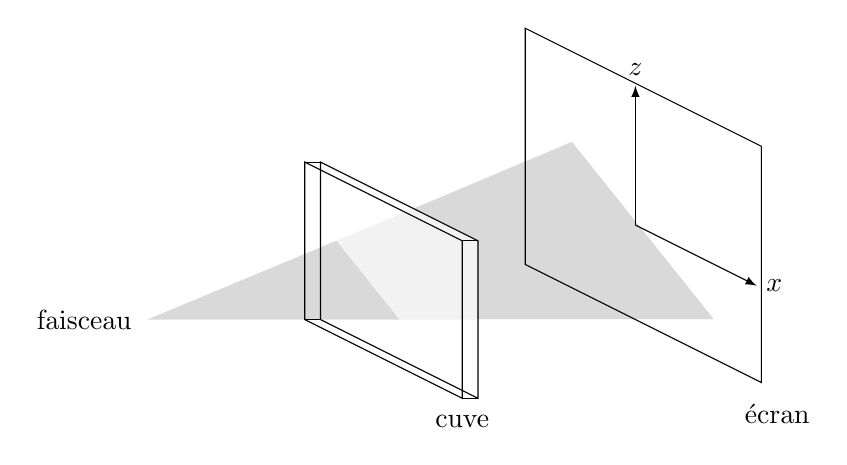
\begin{tikzpicture}

\draw (0,0) --++(2,-1) --++(0,-2) --++(-2,1) --cycle ;
\draw (0,0) --++(0.2,0);
\draw (0.2,0) --++(2,-1) --++(0,-2) --++(-2,1) --cycle ;
\draw (2,-1) --++(0.2,0);
\draw (2,-3) --++(0.2,0);
\draw (0,-2) --++(0.2,0);
\node at (2,-3.3) {cuve};
\node at (6,-3.2) {\'ecran};
\node at (-2.8,-2) {faisceau};

\draw (2.8,1.7) --++(3,-1.5) --++(0,-3) --++(-3,1.5) --cycle ;
\fill[opacity=0.15] (-2,-2) --++ (2.4,1) --++(0.8,-1) --cycle;
\fill[opacity=0.05] (0.4,-1) --++(0.8,-1) --++ (4,0) -- ++(-1.8,2.25) --cycle;
\fill[opacity=0.1] (1.38,-0.59) --++(0.81,-0.4) --++ (0,-1) --++(3,0) --++(-1.8,2.25) --cycle;
\draw[->,>=latex] (4.2,-0.8) --++(0,1.77) node[above] {$z$};
\draw[->,>=latex] (4.2,-0.8) --++(1.54,-0.77) node[right] {$x$};

\end{tikzpicture}
\end{center}
%\caption{Le faisceau qui traverse la cuve n'est pas diffusé dans un mélange homogène et frappe l'écran situé à une distance $L$ de la cuve avec un angle de $45^\circ$. Lorsque le glycérol est introduit, l'indice optique varie avec l'altitude $z$ dans la cuve et le temps $t$, de sorte que le faisceau est dévié vers le bas.}
%\label{fig:pince}
%\end{figure}

\begin{quest}

\item Rappeler la loi de Fick. À partir d'un bilan de matière, montrer que la concentration $c(z,t)$ vérifie l'équation de diffusion $1$D,
\begin{equation}
\label{eq:diff}
\dr{c}{t} = D \drm{c}{z}{2},
\end{equation}
avec $D$ le coefficient de diffusion.
\item Montrer que l'angle de déviation $\theta(z,t)$ vérifie aussi l'Éq.~\eqref{eq:diff}.

\item Vérifie qu'une fonction de la forme $\theta(z,t) = -A \frac{e^{-z^2/4Dt}}{\sqrt{4 \pi Dt}}$ est solution de l'Éq.~\eqref{eq:diff}.

\item On suppose que l'interface est parfaitement plane à $t=0$, et donc que la concentration en glycérol vaut $c(z,t=0)=0$ si $z>0$ et $c(z,t=0)=1$ si $z<0$. À partir de ces conditions initiales, montrer que $A=e(n_g-n_e)$.


\item En présence de pesanteur, le courant de particule vaut $\vec{j} = -D \, \vec{\text{grad}} \, c + \alpha mc \vec{g}$, où $\alpha$ est une constante et $m$ la masse d'une molécule. À partir d'un bilan de matière, montrer que la concentration satisfait à l'équation
\begin{equation}
\dr{c}{t} = D \drm{c}{z}{2} + \alpha mg \dr{c}{z}.
\end{equation}
Déterminer le profil de concentration une fois le régime permanent atteint.\\

Mesure du coefficient de diffusion.

\item On suppose à nouveau que la pesanteur est négligeable. Soit $z_0(x)$ le graphe de la trace du faisceau sur l'écran. Avant d'introduire le glycérol, la trace du faisceau sur l'écran est la droite d'équation $z_0(x)=x$. Montrer qu'en supposant $\theta \ll 1$, la trace du faisceau après ajout de glycérol est
\begin{equation}
z_0(x) = x- e(n_g-n_e)L \ \frac{e^{-x^2/4Dt}}{\sqrt{4 \pi Dt}}.
\end{equation}
Montrer que l'abscisse pour laquelle la distance à la droite d'équation $z_0(x)=x$ est maximale est en $x=0$.
%Déterminer également l'abscisse $x_m(t)$ pour laquelle la hauteur du faisceau sur l'écran est minimale. Interpréter graphiquement.

\item Soit $h(t)$ la hauteur entre la droite d'équation $z=x$ et la trace du faisceau $z_0(x)$ en $x=0$. Montrer que $1/h^2$ est proportionnel au temps $t$.

\sol{pente
$\frac{4 \pi D}{(eL(n_g-n_e))^2}$}

\end{quest}
\end{exo}
%%%%%%%%%%%%%%%%%%%%%%%%%%%%%%%%%%%%%%%%%%%%%%%%%%%%%%%%%%%%%%%%%


%%%%%%%%%%%%%%%%%%%%%%%%%%%%%%%%%%%%%%%%%%%%%%%%%%%%%%%%%%%%%%%%%
\begin{exo}[PC][1][colle]{Marche aléatoire et propriétés de la diffusion}%{1}
On souhaite modéliser le mouvement brownien, à l'origine physique du phénomène de diffusion. On considère un gaz parfait monoatomique d'atomes d'argon Ar de masse molaire $M = \SI{40}{g.mol^{-1}}$ à la température ambiante $T=\SI{300}{K}$.  On note $R$ la constante des gaz parfaits. Le libre parcours moyen vaut $\ell = \SI{100}{nm}$.
 \begin{quest}
  \item
  Par analyse dimensionnelle, déterminer et calculer numériquement la vitesse moyenne $v$ des atomes suite à leur agitation thermique. De même, exprimer le coefficient de diffusion $D$ en fonction de $v$ et $\ell$. Application numérique.
  Calculer le temps $t$ que mettrait le gaz pour diffuser sur une distance $\delta = \SI{2.5}{m}$.
  \sol{$v\sim \sqrt{\frac{RT}{M}}$}
\end{quest}
On modélise l'agitation des atomes du gaz par un marcheur aléatoire sur un axe $(Ox)$. À chaque pas de temps $\tau$, le marcheur à la position $x$ saute soit à gauche à la position $x-\ell$, soit à droite à la position $x+\ell$, avec la même probabilité.
Soit $p(x_n,t_m)$ la probabilité que le marcheur ait effectué globalement $n$ pas vers la droite après $m$ sauts.
  \begin{quest}
 \item Justifier que $p(x_n,t_{m+1}) = \frac{1}{2} p(x_{n-1},t_m) + \frac{1}{2} p(x_{n+1},t_m) $.
 \item
 Montrer que si l'on suppose que la fonction $p(x,t)$ varie \guill{lentement}, elle vérifie une équation de diffusion
$$
   \dr{p}{t} = D \drm{p}{x}{2}.
$$
Exprimer le coefficient de diffusion $D$ en fonction de $\ell$ et $\tau$.
\sol{
$D = \frac{\ell^2}{2 \tau}$
}
\item Proposer un algorithme puis un programme python pour simuler cette marche aléatoire.
\end{quest}
\end{exo}
%%%%%%%%%%%%%%%%%%%%%%%%%%%%%%%%%%%%%%%%%%%%%%%%%%%%%%%%%%%%%%%%%

%%%%%%%%%%%%%%%%%%%%%%%%%%%%%%%%%%%%%%%%%%%%%%%%%%%%%%%%%%%%%%%%%%
%\begin{exotd}[PC]{Diffusion de particules entre deux solutions}{1}
%On considère une cuve parallélépipédique de dimension longitudinale $z$ grande devant ses dimensions transverses. Cette cuve est remplie d'un liquide contenant les mêmes particules, mais elle est séparée en deux parties égales en $z=0$ par une paroi. Au départ, les concentrations sont homogènes, mais différentes de part et d'autre de la paroi: $c_1$ pour $z<0$ et $c_2$ pour $z>0$. À $t=0$ on retire la paroi et les particules diffusent selon la loi de Fick: on notera la concentration locale dans la cuve $c(z,t)$.
%Très loin de la paroi, on a les conditions aux limites $\forall t, c(-\infty,t)=c_1$ et $c(\infty,t)=c_2$.
%\begin{quest}
%\item Vérifier que $g(u)=\frac{2}{\sqrt{\pi}}\int_{0}^{u}\e^{-y^2}\d y$ où $u=\frac{z}{2\sqrt{Dt}}$ est solution de l'équation de diffusion.
%\item Justifier que l'on puisse choisir $c(z,t)=Ag(u)+B$ dans toute la cuve (pour les deux domaines en $z<0$ et $z>0$) avec les \textbf{mêmes} constantes $A$ et $B$, que l'on déterminera.
%\item Tracer l'allure de $c(z,t)$ à $t=0$ puis à deux temps ultérieurs $t_1$ et $t_2>t_1$.
%\item En supposant que l'indice de réfraction $n$ du milieu peut s'écrire comme une fonction affine de la concentration $n(z,t)=n_0+\eta c(z,t)$, exprimer le gradient d'indice et en déduire une méthode physique pour déterminer le coefficient de diffusion $D$.
%\end{quest}
%\end{exotd}
%%%%%%%%%%%%%%%%%%%%%%%%%%%%%%%%%%%%%%%%%%%%%%%%%%%%%%%%%%%%%%%%%%

%%%%%%%%%%%%%%%%%%%%%%%%%%%%%%%%%%%
\begin{exo}[PC][1][colle]{Diffusion d'électrons dans un métal}
  La conduction électrique dans un métal est décrite par le modèle de Drude. Les électrons de conduction d'un métal, présents avec une densité particulaire $n(M,t)$, subissent une force de friction phénoménologique de la forme $\Vec{F} = -m\gamma \Vec{v}$, où $m$ est la masse d'un électron, $\gamma$ le coefficient de friction, et $\Vec{v}$ la vitesse d'un électron. On applique un champ électrique uniforme $\E$ dans le métal.
  \begin{quest}
    \item	En appliquant le PFD à un électron, montrer qu'en régime quasi-permanent la vitesse limite de l'électron vaut $\Vec{v} = -\gamma e  \E$, où $e$ désigne la charge élémentaire. En déduire le vecteur densité de courant de particules $\j_{\!c}$ due au phénomène de conduction.
    \item Rappeler l'expression de la densité de courant de particules $\j_{\!d}$ due au phénomène de diffusion, donnée par la loi de Fick. Que vaut le vecteur densité de courant de particules total $\Vec{\jN}$ ?
    \item À partir de l'équation de conservation de la matière, 
    $$
    \dr{n}{t} + \dive{\Vec{\jN}} =0,
    $$
    déterminer l'équation vérifiée par la densité particulaire $n(M,t)$. On suppose que le champ électrique est de la forme $\E = E \ex$ avec $E>0$ une constante et que la densité particulaire ne dépend que de la coordonnée spatiale $x$. Que vaut $n(x)$ en régime permanent sachant qu'à l'extrémité $x=0$ du métal, $n(x=0)=n_0$ ?
  \end{quest}

\end{exo}
%%%%%%%%%%%%%%%%%%%%%%%%%%%%%%%%%%%


%%%%%%%%%%%%%%%%%%%%%%%%%%%%%%%%%%%%%%%%%%%%%%%%%%%%%%%%%%%%%%%%%
\begin{exo}[PC][3][TD]{Diffusion du glycérol dans l'eau}
  \Notions{\item Équation de diffusion \task Régime transitoire}
  \Annale[Physique PSI]{E3A}{2012}
On considère une cuve parallélépipédique de hauteur et de largeur grande devant son épaisseur~$e$. La cuve, posée verticalement, contient un fond de glycérol, dont la surface est à l'altitude $z=0$.  On notera $c(z,t)$ la densité particulaire en glycérol dans la cuve. À l'instant $t=0$, on dépose doucement de l'eau liquide sur la surface de glycérol : la concentration en glycérol vaut alors $c(z,t=0) = c_0$ pour $z<0$ et $c(z,t=0)=0$ pour $z>0$.
Ensuite, les liquides diffusent l'un dans l'autre selon la loi de Fick.
Très loin de la paroi, les conditions aux limites sont $c(z=-\infty,t)=c_0$ et $c(z=\infty,t)=0$ pour tout $t$. Le schéma de l'expérience est représenté sur la \Fig{diffu_imag}.
\begin{fig}[label]
  \centering
  
\includegraphics[width=0.7\columnwidth]{schema_exp_glycerol_final.pdf}
  %\capt{}
\end{fig}
\begin{quest}
\item Écrire l'équation de diffusion pour la concentration $c(z,t)$. On cherche une solution auto-similaire : on suppose que la densité $c(z,t) = g(u)$ ne dépend que de la variable $u=\frac{z}{2\sqrt{Dt}}$. D'après les propriétés des phénomènes diffusifs, pourquoi est-il naturel de chercher une solution de cette forme ?

\sol{L'équation de diffusion s'écrit
$$
\dr{c}{t} = D\drm{c}{z}{2}.
$$
Les processus diffusifs se propagent sur une distance \fbox{$\delta \propto \sqrt{Dt}$}.
Un front de diffusion donné est donc tel que le rapport $u=z/\sqrt{2Dt}$ est constant au cours de son évolution.
Il est donc naturel de pouvoir se ramener cette seule variable $u$.
}


\item Monter que $g$ vérifie l'équation
 \begin{equation}\label{eq:diffu_g}
 \ddm{g}{u}{2} =  -2u \dd{g}{u}.
 \end{equation}
 \sol{
 On a $$\dr{c}{t} = \dr{u}{t} \dd{g}{u} = -\frac{1}{4\sqrt{D}t^{3/2}} \dd{g}{u}$$ et $$\dr{c}{z} = \frac{1}{2\sqrt{Dt}}\dd{g}{u},$$ d'où l'on tire
 \eqbox{\drm{c}{z}{2} = \frac{1}{4Dt}\ddm{g}{u}{2}.}
 }


\item Vérifier que $g(u)= A\, \text{erf}(u) + B$ est solution de l'\Eq{diffu_g}, où l'on a défini la fonction erreur de Gauss 
\begin{equation}
\text{erf}(u) = \frac{2}{\sqrt{\pi}} \int_{0}^{u}\e^{-y^2}\d y.
\end{equation}
Déterminer les constantes $A$ et $B$ telles que $c(z,t)= g(u)$ vérifie les conditions aux limites. Que dire de la condition initiale ?

\sol{
Par définition de l'intégrale, $\dd{g}{u} = A e^{-u^2}$ et donc
$$
\ddm{g}{u}{2} =(-2u) A e^{-u^2} = -2u \dd{g}{u}.
$$
\underline{Condition initiale}.
On trouve pour $t=0^+$ que
\begin{liste}
  \item si $z>0$, alors $u=+\infty$ et donc $\int_0^\infty e^{-y^2} \d y =  \frac{\sqrt{\pi}}{2}$ ;
  \item si $z<0$, alors  $u=-\infty$ et donc $\int_0^{-\infty} e^{-y^2} \d y = -\frac{\sqrt{\pi}}{2}$.
\end{liste}
On a donc
$$\left\{
\begin{array}{lll}
c(z>0,t=0) & = 0 & = A\frac{\sqrt{\pi}}{2} + B \\
c(z<0,t=0) & = c_0 & = -A\frac{\sqrt{\pi}}{2} + B \\
\end{array}\right.
$$
soit $B = - \frac{\sqrt{\pi}}{2} A = \frac{c_0}{2}$ et $A = -\frac{c_0}{\sqrt{\pi}}$. En conclusion,
\eqbox[*]{c(z,t) = -\frac{c_0}{\sqrt{\pi}} \int_{0}^{\frac{z}{2\sqrt{Dt}}}\e^{-y^2}\d y + \frac{c_0}{2}.}
Pour $z=+\infty$ à $t$ fini, on trouve $u=+\infty$, et pour $z=-\infty$ à $t$ fini, $u=-\infty$ ; les conditions aux limites sont donc vérifiées.
}
%\item Justifier que l'on puisse choisir $c(z,t)=Ag(u)+B$ dans toute la cuve (pour les deux domaines en $z<0$ et $z>0$) avec les \textbf{mêmes} constantes $A$ et $B$, que l'on déterminera.
\item Tracer l'allure de $c(z,t)$ à $t=0$ puis à deux temps ultérieurs $t_1$ et $t_2>t_1$.
\sol{
  On peut tracer deux courbes similaires aux courbes expérimentales observées sur la figure \Fig{diffu_imag}.
}
\item En supposant que l'indice de réfraction $n(z,t)$ du mélange liquide est une fonction affine de la densité en glycérol, $n(z,t)=n_0+a\, c(z,t)$, calculer le gradient d'indice $\dr{n}{z}(z,t)$.
\sol{
  On a 
  \eqbox{
  \dr{n}{z}(z,t) = a \dr{c}{z}(z,t) = \frac{a c_0}{2\sqrt{\pi D t}} \e^{-\frac{z^2}{4Dt}.}
  }
}
\item On peut montrer que la déviation du faisceau sur un écran situé derrière la cuve à une distance $L$ s'écrit $h(t)\simeq L \dr{n}{z}(z=0,t)$ pour de petits angles de déviation. Montrer que la fonction $h(t)$ a pour expression
\begin{equation}
  h(t)\simeq  \frac{aL c_0}{2\sqrt{\pi D t}}.
\end{equation}
En déduire une méthode optique pour mesurer le coefficient de diffusion $D$ du glycérol et expliquer les photos de la \Fig{diffu_imag}.
\sol{
  On a 
  \eqbox{
  h(t)\simeq L\dr{n}{z}(z=0,t) = \frac{aL c_0}{2\sqrt{\pi D t}}.
  }
Envoyons un faisceau laser à travers la cuve. L'angle de déviation des rayons en sortie de la cuve est proportionnelle est gradient d'indice.
\begin{center}

\includegraphics[scale=1]{deviation.pdf}
\end{center}
On observe donc un profil gaussien de déviation du faisceau sur un écran placé  à une distance $L$. La hauteur maximale du profil gaussien $h(t)$ varie comme $1/\sqrt{t}$.
% \begin{center}
% 
\includegraphics[scale=1]{schema_exp_glycerol_final.pdf}
% \end{center}
}

\end{quest}
\begin{fig}[diffu_imag]
    \renewcommand\thesubfigure{}
\centering
\begin{subfig}[label][0.15]
  
\includegraphics[scale=0.45]{c_t=0h_final.pdf}
\end{subfig}
\begin{subfig}[label][0.15]
  
\includegraphics[scale=0.45]{c_t=1h_final.pdf}
\end{subfig}
\begin{subfig}[label][0.15]
  
\includegraphics[scale=0.45]{c_t=2h_final.pdf}
\end{subfig}
\begin{subfig}[label][0.15]
  
\includegraphics[scale=0.45]{c_t=3h_final.pdf}
\end{subfig}
\begin{subfig}[label][0.15]
  
\includegraphics[scale=0.45]{c_t=4h_final.pdf}
\end{subfig}
% \subfigure[\large{\small  $t_{\rm exp}=\SI{0}{h}$}]{
\includegraphics[scale=0.45]{c_t=0h_final.pdf}}\hfill
% \subfigure[\large{\small $t_{\rm exp}=\SI{1}{h}$}]{
\includegraphics[scale=0.45]{c_t=1h_final.pdf}}\hfill
% \subfigure[\large{\small $t_{\rm exp}=\SI{2}{h}$}]{  
\includegraphics[scale=0.45]{c_t=2h_final.pdf}}\hfill
% \subfigure[\large{\small $t_{\rm exp}=\SI{3}{h}$}]{
\includegraphics[scale=0.45]{c_t=3h_final.pdf}}\hfill
% \subfigure[\large{\small $t_{\rm exp}=\SI{4}{h}$}]{
\includegraphics[scale=0.45]{c_t=4h_final.pdf}}
  \capt{%Profil
  Trace lumineuse sur l'écran aux instants (a) $t_{\rm exp}=\SI{0}{h}$, (b) $t_{\rm exp}=\SI{1}{h}$, (c) $t_{\rm exp}=\SI{2}{h}$, (d) $t_{\rm exp}=\SI{3}{h}$ et (e) $t_{\rm exp}=\SI{4}{h}$ depuis le début de l'expérience.
   La hauteur du rectangle blanc représente $\SI{10}{cm}$ et s'applique aux échelles verticale et horizontale. La distance $h(t)$ entre le profil du faisceau non dévié (droite jaune tiretée) et le profil instantané (croix jaune) se mesure le long de la verticale passant par le point initialement le plus bas (droite continue blanche).\label{fig:profils}}
\renewcommand\thesubfigure{(\alph{subfigure})}
\end{fig}

\begin{fig}[h_vs_t]
\centering

\includegraphics[scale=1.1]{hauteur_vs_texp_inset.pdf}
\capt{Hauteur $h$ en fonction du temps $t_{\rm exp}$ depuis le début de la série de mesures.
% Une régression affine du temps écoulé en fonction de $1/h^2$ donne $t_{\rm exp}=a/h^2+b$ avec $b=-\SI{49.9(4)}{min}$ et $a = \SI{1.785(9)e2}{s.m^2}$.
}
\end{fig}


\begin{quest}
  \item  On a représenté en \Fig{diffu_imag} et \Fig{h_vs_t} les résultats d'une expérience de diffusion d'un mélange eau-glycérol à $\SI{50}{\%}$ en masse dans l'eau. Déterminer le coefficient de diffusion $D$ à partir des mesures, sachant que $ac_0 = \SI{7.3e-4}{m}$ et $L=\SI{1.5}{m}$.
  \sol{
    On lit sur le graphe que la loi $t_{\rm exp} = c/h^2+d$ est bien vérifiée avec $c\simeq \SI{5e-2}{s.m^2}$. On en déduit le coefficient de diffusion
    \eqbox{
      D = \frac{(ac_0 L)^2}{4\pi c} = \SI{5.3e-10}{m^2.s^{-1}}
    }
  }
\end{quest}
\end{exo}
%%%%%%%%%%%%%%%%%%%%%%%%%%%%%%%%%%%%%%%%%%%%%%%%%%%%%%%%%%%%%%%%%

%%%%%%%%%%%%%%%%%%%%%%%%%%%%%%%%%%%%%%%%%%%%%%%%%%%%%%%%%%%%%%%%%
\begin{exo}[PC][2][TD]{Diffusion de neutrons dans un réacteur nucléaire}
  \Notions{\item Diffusion \task Terme de production \task Régime transitoire \task Géométrie unidimensionnelle}
On étudie la diffusion de neutrons dans la matière fissile d'un réacteur nucléaire assimilé à un cylindre de section $S$ constante situé entre les plans d'abscisses $x=0$ et $x=a$. Le réacteur est homogène. On note $n(x,t)$ la densité volumique de neutrons et $\Vec{\jN}=\jN(x,t)\,\ex$ le vecteur densité de courant de neutrons. On donne le coefficient de diffusion $D=\SI{20}{m^2.s^{-1}}$.


\begin{center}

\includegraphics[scale=0.7]{diffusion_1D_cylindre.pdf}
\end{center}
%On suppose que le milieu dans lequel évoluent les neutrons est homogène et contient $N$ atomes de plutonium par unité de volume ($N=\cte$). On suppose pour simplifier que tous les neutrons ont des vitesses de même module moyen $v$. On désigne par $n(M,t)$ le nombre de neutrons par unité de volume en un point $M$ à l'instant $t$; $\vec{j}(M,t)$ le vecteur densité de courant de particules en $M$ à l'instant $t$; $D$ le coefficient de diffusion. Le réacteur est sphérique, de centre $O$ et de rayon $a$, et on admet que $\vec{\jN}=j(r,t)\,\vec{e}_r$ et $n=n(r,t)$.
\begin{quest}
\item À chaque collision avec un noyau, un neutron a une probabilité $\alpha = \num{0.3}$ d'être absorbé par un noyau. La durée de vie moyenne d'un neutron vaut $\tau=\SI{4.2e-5}{s}$.
On considère un tronçon élémentaire de matière fissile de volume $\d V = S \d x$.
Justifier que le nombre moyen de neutrons absorbé par unité de temps et de volume vaut $p_{\rm abs} =  \frac{\alpha}{\tau} n$.

\sol{
Le nombre de neutrons dans ce tronçon vaut $\d N = n \d V$.
En moyenne, un neutron entre en collision une fois tous les $\tau$, donc le nombre de neutrons qui entrent en collision dans ce volume vaut, par unité de temps, $\d \Phi_{\rm coll} = \frac{\d N}{\tau} = \frac{n}{\tau} \d V$.
Chaque collision mène à une absorption avec une probabilité $\alpha$, donc le nombre de neutrons absorbés dans ce volume vaut, par unité de temps, $\d \Phi_{\rm abs} = \alpha\, \d \Phi_{\rm coll} =  \frac{\alpha n}{\tau} \d V$.
On divise ce flux absorbé par le volume pour obtenir
\eqbox[*]{p_{\rm abs} =  \frac{\alpha n}{\tau}.}
}


\item Pour chaque neutron absorbé, le noyau percuté fissionne et produit une moyenne de $K=\num{2,75}$ neutrons. Justifier que le nombre de neutrons produits par unité de temps et de volume vaut $p_{\rm prod} = \frac{\alpha (K-1)}{\tau} n$.
Effectuer un bilan du nombre de neutrons sur un tronçon élémentaire de matière fissile d'épaisseur $\d x$.
En déduire que $n(x,t)$ vérifie l'équation différentielle
\begin{equation}
\dr{n}{t} = D \drm{n}{x}{2} + \frac{\alpha(K-1)}{\tau}n.
\end{equation}

\sol{
Chaque neutrons absorbé conduit à $K$ neutrons produits, donc la variation du nombre de neutrons à chaque absorption vaut $K-1$. On en déduit que $p_{\rm prod} = (K-1)p_{\rm abs}=\frac{\alpha(K-1)}{\tau}n$.


La variation $\d N$ du nombre de neutrons pendant $\d t$ vaut
$$
\d N = [n(x,t+d t)-n(x,t)]S\d x  = \dr{n}{t} \d t S \d x
$$
En faisant le bilan de ce qui entre, ce qui sort, et ce qui est produit, on obtient
$$
\d N = \underbrace{\jN(x,t) S \d t}_{\rm entrée} -\underbrace{\jN(x+\d x,t) S \d t}_{\rm sortie} + \underbrace{p_{\rm prod} \d V \d t}_{\rm produit} \simeq \left[-\dr{\jN}{x}(x,t) + p_{\rm prod}\right]\d t S \d x.
$$
D'après la loi de Fick, $\Vec{\jN} = -D \,\grad n$ et donc
\eqbox{\dr{n}{t} = -\dr{\jN}{x}(x,t) + p_{\rm prod} = D \drm{n}{x}{2} + \alpha(K-1)\frac{n}{\tau}.}
}

\item En régime permanent, déterminer $n(x)$ en supposant $n(x=a)=n(x=0)=0$. Déterminer la longueur d'onde $\lambda_0$ des oscillations des densités. Que vaut la taille $a$ du réacteur ? \AN ? 

\sol{
On obtient l'équation d'un oscillateur harmonique,
$$\ddm{n}{x}{2} + \frac{\alpha(K-1)}{\tau D} n  =0.$$
La solution est sinusoïdale, de la forme $n(x) = A \cos(k_0 x) + B \sin(k_0 x)$ avec $k_0^2 = \frac{\alpha(K-1)}{D\tau}$. La longueur d'onde des oscillations vaut
\eqbox{\lambda_0 = \frac{2\pi}{k_0} = 2\pi \sqrt{\frac{D \tau}{\alpha(K-1)}}.}
Les conditions initiales imposent $n(x=0) = A = 0$ et $n(x=a) = B \sin(k_0 a) = 0$. La seconde égalité nous donne soit $B=0$ (mais alors $n=0$ partout, ce qui n'est pas intéressant), soit $\sin(k_0 a)=0$.
Alors $k_0 a = m \pi$ avec $m$ entier. Mais comme $n>0$ par définition, la seule solution physique est $m=1$. Cela impose que la taille $a$ du système soit reliée aux autres grandeurs
\eqbox{a = \frac{\lambda_0}{2} = \pi \sqrt{\frac{D \tau}{\alpha(K-1)}}.}
On remarque que $B$ est indéterminé. \AN~: $\lambda_0 = \SI{25}{cm}$ et $a = \SI{13}{cm}$.
}

\item On cherche maintenant une solution décroissante dans le temps sous la forme $n(x,t)=f(x)\,\e^{-t/T}$. On impose les mêmes conditions aux limites qu'auparavant, soit $n(x=a,t)=n(x=0,t)=0$. On prend pour condition initiale $n(x,t=0) = n_0 \sin(2\pi \frac{x}{\lambda})$, où $\lambda$ est la longueur d'onde initiale des oscillations de densité.
 Déterminer $f(x)$, $\lambda$, et $T$, puis discuter de la nature du régime transitoire en fonction de la taille $a$ du réacteur. Que vaut numériquement $T$ pour $a=\SI{10}{cm}$ ?

\sol{
On obtient avec l'équation de diffusion
$$
-\frac{1}{T} \e^{-t/T} f(x) = \e^{-t/T} \left[ D \ddm{f}{x}{2}(x) + \frac{\alpha(K-1)}{\tau} f(x) \right] \Rightarrow  \ddm{f}{x}{2} +\left( \frac{\alpha(K-1)}{\tau D} + \frac{1}{DT}\right) f = 0.
$$
Le nouveau vecteur d'onde $k$ est tel que $k^2 = \frac{\alpha(K-1)}{\tau D} + \frac{1}{DT}$. Les conditions aux limites sont les mêmes, et donc
$$
n(x,t) = n_0 \, \e^{-t/T}  \sin(k x).
$$
La condition en sortie du réacteur impose aussi $n(a,t) = 0$, soit $\sin(k a)=0$ et donc à nouveau $ka = \pi$. La période de décroissance $T$ doit donc vérifier
$$
\frac{\alpha(K-1)}{D\tau} + \frac{1}{DT} = k^2 = \frac{\pi^2}{a^2} \Rightarrow T = \left[\frac{D \pi^2}{a^2}  - \frac{\alpha(K-1)}{\tau} \right]^{-1}.
$$
soit
\eqbox{T=\frac{\tau}{\alpha(K-1)} \left[\frac{\lambda_0^2}{4a^2}  -  1\right]^{-1} .}
En régime transitoire sous-critique (décroissance exponentielle) $T>0$ et $a$ n'est pas contraint. Pour avoir un régime permanent non trivial, il faut $T=\infty$ et donc on retrouve la condition précédente $a=\frac{\lambda_0}{2}$ : il s'agit du régime critique.
Si $a>\frac{\lambda_0}{2}$, alors $T<0$ et le régime transitoire est sur-critique (croissance exponentielle et explosion !). \AN~: pour $a=\SI{10}{cm}$, on trouve $T=\SI{1.4}{ms}$.

}
\end{quest}
\end{exo}
%%%%%%%%%%%%%%%%%%%%%%%%%%%%%%%%%%%%%%%%%%%%%%%%%%%%%%%%%%%%%%%%%
